\documentclass[11pt]{article}

\usepackage[margin=1in]{geometry}
\usepackage{ifxetex}
\ifxetex
  % XeLaTeX (tectonic, lokal)
  \usepackage{fontspec}
  \setmainfont{lmroman10-regular.otf}[
    BoldFont=lmroman10-bold.otf,
    ItalicFont=lmroman10-italic.otf,
    BoldItalicFont=lmroman10-bolditalic.otf,
  ]
  \setsansfont{lmsans10-regular.otf}[
    BoldFont=lmsans10-bold.otf,
    ItalicFont=lmsans10-oblique.otf,
  ]
  \setmonofont{lmmono10-regular.otf}
\else
  % pdfLaTeX (Overleaf)
  \usepackage[T1]{fontenc}
  \usepackage[utf8]{inputenc}
  \usepackage{lmodern}
\fi
\usepackage[english]{babel}
\usepackage{amsmath,amssymb}
\usepackage{graphicx}
\usepackage{grffile}
\usepackage{float}
\usepackage{booktabs}
\usepackage{array}
\usepackage[authoryear,round]{natbib}
\usepackage{url}
\usepackage{hyperref}
\usepackage{caption}
\usepackage{setspace}
\usepackage{framed}
\usepackage{xcolor}

\setlength{\parindent}{0pt}
\setlength{\parskip}{0.8\baselineskip}
\emergencystretch=2em

\hypersetup{
    colorlinks=true,
    linkcolor=black,
    citecolor=blue!60!black,
    urlcolor=blue!60!black,
}

% --- kisaltmalar ---
\newcommand{\ltyirmi}{$<\!20\%$}
\newcommand{\fairs}{\textit{fairness\_salience}}
\newcommand{\disp}{\textit{disposable\_income\_buffer}}

% --- finding / verdict kutulari ---
\definecolor{shadecolor}{rgb}{0.96,0.96,0.96}
\newenvironment{findingbox}{%
    \begin{shaded}\noindent\textbf{BULGU.}\quad}{\end{shaded}}

\newcommand{\verdictbox}[1]{%
    \begin{center}
    \fbox{\parbox{0.92\linewidth}{\centering\textbf{#1}}}
    \end{center}}


\title{\textbf{LLM'ler kültürü değil, kültürün tarifini simüle ediyor}\\[0.3em]
\large Ültimatom Oyununda Henrich'in bulgusunu yeniden üretme denemesi}

\author{Gökhan Geyik\\\textit{Empler AI}\\\texttt{gokhan@empler.ai}\\ORCID: \href{https://orcid.org/0009-0000-9028-1827}{0009-0000-9028-1827}}

\date{Ekim 2026}

\begin{document}

\renewcommand{\abstractname}{Öz}
\renewcommand{\refname}{Kaynakça}
\renewcommand{\figurename}{Şekil}
\renewcommand{\tablename}{Tablo}

\maketitle

\textbf{Anahtar Kelimeler:} Ültimatom oyunu $\cdot$ büyük dil modelleri $\cdot$ üretici ajan tabanlı modelleme $\cdot$ kültürlerarası davranış $\cdot$ WEIRD $\cdot$ persona simülasyonu $\cdot$ istem duyarlılığı $\cdot$ replikasyon

\begin{abstract}
\noindent
Büyük dil modellerine (LLM) bir kültürel kimlik tarif edip onları insan katılımcıların yerine kullanmak, üretici ajan tabanlı modellemede (GABM) giderek yaygınlaşan bir yöntemdir. Bu çalışma yöntemin geçerliliğini, davranışsal ekonominin en iyi belgelenmiş kültürlerarası bulgularından biri üzerinden sınamaktadır: Ültimatom Oyununda düşük teklifleri WEIRD öğrencilerin sık (\%40--60), piyasa entegrasyonu düşük birçok küçük ölçekli toplulukta ise düşük tekliflerin nadiren reddedilmesi. Üç model ailesi (Claude Haiku 4.5, Gemma-4-31b-it, GPT-OSS-120b) ile, her adımının hipotezleri ve analiz planı veri toplanmadan önce yazılı olarak dosyalanmış ardışık bir inceleme yürütülmüştür. Aynı kişiler, aynı oyun ve aynı teklifler için sonuç yalnızca kimlik tarifinin yazılışına göre kökten değişmiştir. Tarife klasik ajan tabanlı modelleme geleneğine uygun olarak sayısal bir ``adalet önemi'' puanı eklendiğinde (Çalışma~1) modeller \%10'luk teklifleri yalnızca \%3 oranında reddetmiştir; aynı kartta puanın 0,3'ten 0,6'ya çıkması düşük tekliflerde reddetmeyi üç modelde \%5'ten \%52'ye yükseltmiştir. Sayılar kaldırıldığında (Çalışma~2) Henrich'in bulgusunun \emph{tersi} bir fark ortaya çıkmıştır: küçük ölçekli kartlar \%61, WEIRD kartları \%6 oranında reddetmiştir (üç modelde de aynı yön). Ancak bu ters fark yalnızca tarifte ``karşılıklılık, paylaşım, akrabalık ağı'' gibi değer yüklü ifadeler bulunduğunda görülmüştür; kimlik yalnızca yaş ve meslekle ya da topluluk büyüklüğünü ve piyasa entegrasyonunu olgusal olarak anlatan bir metinle tarif edildiğinde kollar arasında fark kalmamıştır (\%21'e karşı \%24; \%13'e karşı \%9). Hiçbir tarifte Henrich'in gözlediği örüntü üretilmemiştir. Bulgular, kimlik tarifiyle yönlendirilen LLM ajanlarının simüle edilen kültürün davranışını değil, o kültürün nasıl tarif edildiğini yansıttığını göstermektedir; tariflere eklenen sayısal ve değer yüklü ifadeler kültürlerarası sonucun hem varlığını hem yönünü belirleyebilmektedir.
\end{abstract}


\section{Giriş}

Ültimatom Oyunu \citep{guth1982} yalın bir pazarlık durumudur: bir teklif edici 100 birimlik bir havuzdan karşı tarafa bir pay önerir; yanıtlayıcı kabul ederse iki taraf paylarını alır, reddederse ikisi de sıfır kazanır. Kendi çıkarını en üst düzeye çıkaran bir yanıtlayıcı sıfırdan büyük her teklifi kabul etmelidir; oysa insan katılımcılar düşük teklifleri düzenli olarak reddeder. \citet{henrich2001} 15 küçük ölçekli toplulukta yürüttükleri saha deneyleriyle bu davranışın kültürler arasında büyük farklılık gösterdiğini ortaya koymuştur: WEIRD (Batılı, Eğitimli, Sanayileşmiş, Zengin, Demokratik) üniversite öğrencileri havuzun \%20'sinin altındaki teklifleri \%40--60 oranında reddederken, piyasa entegrasyonu düşük birçok toplulukta düşük teklifler neredeyse hiç reddedilmemiştir: Peru Amazonlarındaki Machiguenga'da tekliflerin çoğu düşük olduğu halde yalnızca bir teklif reddedilmiş, Tsiman\'e'de hiçbir teklif reddedilmemiştir. Bu bulgu, adalet normlarının evrensel olmadığının en çok atıf alan kanıtlarından biridir \citep{henrich2010}.

Son yıllarda LLM'lerin insan katılımcıların ``silikon'' vekilleri olarak kullanılması hızla yaygınlaşmıştır \citep{argyle2023,horton2023,aher2023,park2023}. Kültürlerarası çalışmalar için bu yaklaşım özellikle caziptir: bir LLM'ye ``sen Amazon'da geçimlik tarım yapan birisin'' demek, saha çalışmasının maliyetinin küçük bir kesrine mal olur. Bu yaklaşımın temel varsayımı, bir kimlik tarifiyle yönlendirilen modelin o kimliğe sahip gerçek insanların davranışını yansıttığıdır. LLM'lerin kimlik gruplarını düzleştirdiğine ve karikatürleştirdiğine \citep{cheng2023compost,wang2025misportray}, psikolojilerinin WEIRD popülasyonlara benzediğine \citep{atari2023which} ve istem yazımındaki anlamsız değişikliklere aşırı duyarlı olduklarına \citep{sclar2024quantifying} dair bulgular bu varsayımı sorgulatmaktadır.

Bu çalışma Henrich'in bulgusunu GABM çerçevesinde, üç model ailesiyle yeniden üretmeye çalışmaktadır. Çalışma, başlangıçta tek bir deney olarak tasarlanmıştır. İlk deneyin beklenmedik sonucu ardışık testlerle incelenmiş; her testin hipotezleri ve karar kuralları, bir önceki testin sonucu görüldükten sonra ancak kendi verisi toplanmadan önce yazılı olarak dosyalanmıştır (Bölüm~\ref{sec:prereg}). Makale bu ardışık süreci olduğu gibi raporlamaktadır. Ana iddia, iki doğrudan manipülasyona dayanmaktadır: aynı kimliklerin sayısal niteliklerle ve niteliksiz sunulması (Bölüm~\ref{sec:numbers}) ve aynı kimliklerin üç farklı metinle tarif edilmesi (Bölüm~\ref{sec:wording}). Bulgular şöyle özetlenebilir:

\begin{enumerate}
\item \textbf{Sayısal nitelikler sonucu belirler.} Tarife eklenen bir ``adalet önemi'' puanı reddetme oranını büyük ölçüde belirlemektedir. Bu puanlarla yürütülen ilk deneyde (Çalışma~1) modeller neredeyse hiç reddetmemiştir; bunun büyük ölçüde tariflerdeki düşük puanlardan kaynaklandığı ayrı bir testle gösterilmiştir.
\item \textbf{Değer yüklü sözcükler farkın yönünü belirler.} Sayılar kaldırıldığında (Çalışma~2) Henrich'in bulgusunun tersi bir fark ortaya çıkmıştır. Ancak bu fark, küçük ölçekli kimlik ``karşılıklılık, paylaşım, akrabalık ağı'' gibi ifadelerle tarif edildiğinde ortaya çıkmakta; aynı kimlik yalın ya da olgusal bir dille tarif edildiğinde kaybolmaktadır.
\item \textbf{Hiçbir tarif Henrich'i üretmez.} İnsan verisindeki açıklayıcı değişkenler olan topluluk büyüklüğü ve piyasa entegrasyonu olgusal olarak tarif edildiğinde bile modeller insan örüntüsünü üretmemiştir.
\end{enumerate}

Bu bulgular GABM uygulayıcıları için somut bir uyarı içermektedir: kimlik tarifiyle yönlendirilen bir LLM'nin çıktısı, simüle edilen grubun davranışının değil, araştırmacının o grubu nasıl tarif ettiğinin bir fonksiyonudur.


\section{İlgili Çalışmalar}

\subsection{Ültimatom Oyunu ve Kültürlerarası Değişkenlik}

\citet{guth1982}'in Ültimatom Oyunu'nu tanıtmasından bu yana, binlerce deneysel çalışma reddetme davranışının tutarlılığını ve belirleyicilerini incelemiştir. İlk dalga WEIRD örneklemlerinde yürütülen çalışmalardan oluşmuş; \%20 altı tekliflerin rutin olarak reddedildiğini ve modal teklif düzeyinin \%40--\%50 olduğunu belgelemiştir. Ancak \citet{henrich2001}'in 15 küçük ölçekli toplumda gerçekleştirdikleri eş zamanlı saha deneyleri bu tablonun yanıltıcı bir genelleme olduğunu ortaya koymuştur. Araştırma, Machiguenga gibi toplulukların oldukça düşük reddetme oranlarıyla karakterize edildiğini, Lamalera (Endonezya) gibi diğer toplulukların ise hiper-adil tekliflerle ($>$\%50) göze çarptığını göstermiştir.

\citet{henrich2010} bu bulguları daha geniş bir teorik çerçeveye oturtmuş ve psikoloji araştırmalarındaki örneklemlerin \%96'sının dünya nüfusunun yalnızca \%12'sini barındıran ülkelerden geldiği uyarısında bulunmuştur. ``WEIRD sorunu'' kavramı, modern davranışsal ekonomi ve psikolojide belki de en etkili metodolojik eleştirilerden biridir. Bu eleştiri aynı zamanda GABM gibi metodolojik önerilerin neden önemli olabileceğine de işaret etmektedir: etik, finansal ve pratik engeller, kültürlerarası saha çalışmalarını oldukça zorlaştırmaktadır.

\subsection{LLM'ler silikon denek olarak}

LLM'lerin davranışsal denek vekilleri olarak kullanılma fikri, birkaç farklı araştırma programının birleşmesiyle ortaya çıkmıştır. \citet{binz2023}, GPT-3'ü klasik bilişsel psikoloji görevlerine tabi tutmuş ve Linda problemi ile Wason seçim görevi gibi deneylerde insanlarla nitel olarak benzer, ancak tam çakışmayan örüntüler raporlamıştır. \citet{horton2023} ``Homo silicus'' çerçevesinde LLM'lerin ekonomik ajan simülasyonlarında kullanılabileceğini savunmuş ve birkaç klasik deneysel ekonomi sonucunun nitel olarak yeniden üretilebildiğini göstermiştir; ancak bu çalışma kültürlerarası Ültimatom Oyunu replikasyonuna odaklanmamaktadır. \citet{argyle2023} ise GPT-3'ün uygun demografik koşullandırma ile ABD anket alt gruplarının yanıt dağılımlarını taklit edebildiğini göstermiştir.

\citet{aher2023} bu ajandayı ``Turing deneyleri'' çerçevesinde genişletmiş; Ültimatom Oyunu, Garden Path Sentences, Milgram şok deneyi ve Wisdom of Crowds gibi klasik paradigmalarda LLM'lerin insan bulgularını ne ölçüde yeniden üretebildiğini test etmiştir. Önemli olarak, çalışma bu paradigmalarda başarılı replikasyonlar bildirirken, kültürel profiller arası karşılaştırma yapmamış ve ön kayıtlı bir tasarım kullanmamıştır. \citet{park2023}'ün ``üretici ajanlar'' çalışması ise bellek, yansıma ve planlama bileşenleriyle simüle edilmiş bir kasabada ortaya çıkan sosyal dinamikleri göstererek GABM metodolojisinin mimari temelini kurmuştur.

Daha yakın tarihli bir çalışmada \citet{mei2024}, ChatGPT varyantlarını bir dizi davranışsal oyun ve kişilik ölçümü üzerinde karşılaştırarak bir ``davranışsal Turing testi'' yürütmüş ve özellikle ChatGPT-4'ün çok sayıda insan katılımcının dağılımı içinde kaldığını, fakat ortalama ve modal insan davranışına kıyasla daha kooperatif ve daha özgeci davranma eğilimi gösterdiğini raporlamıştır. Bu bulgu, Çalışma~1'deki ve Çalışma~2'nin WEIRD kolundaki ``insan tabanından daha kabul edici'' gözlemimizle yönsel olarak uyumludur; ancak Çalışma~2'nin küçük ölçekli kolu bunun tersini göstermektedir.

Ancak literatürdeki tablo karışıktır: LLM'lerin aynı oyunda farklı koşullamalar altında farklı yönlerde sapabildiği, model boyutuna ve sıcaklık ayarına duyarlı olabildiği gösterilmiştir. Dahası, mevcut GABM çalışmalarının çok azı (i) ön kayıtlı hipotezler, (ii) çoklu model aileleri ve (iii) çoklu varyans taramalarının üçünü birden kullanmaktadır. Bu metodolojik üçlü, LLM-as-subject iddialarının kırılganlığını değerlendirmek için kritiktir. Mevcut çalışma, Henrich paradigması için tam olarak bu titizlikte bir denetim sunmaktadır.


\subsection{Persona simülasyonları ve grup temsili}

LLM'lerin belirli demografik grupları simüle etme yeteneğine dair tartışma son yıllarda yoğunlaşmıştır. \citet{cheng2023compost}, LLM simülasyonlarının personaları çok boyutlu bireyler olarak değil abartılmış karikatürler olarak üretmeye yatkın olduğunu göstermiş ve bu eğilimi ölçmek için bir çerçeve önermiştir. \citet{wang2025misportray}, insan katılımcıların yerine kullanılan LLM'lerin kimlik gruplarını hem yanlış temsil ettiğini hem de grup içi çeşitliliği düzleştirdiğini analitik ve deneysel olarak göstermiştir. \citet{atari2023which} ise LLM'lerin psikolojik ölçümlerdeki yanıtlarının en çok WEIRD popülasyonlara benzediğini ve WEIRD olmayan toplumlara uzaklaştıkça benzerliğin hızla azaldığını raporlamıştır. Mevcut çalışma bu literatüre davranışsal bir karar paradigmasında, ön kayıtlı ve doğrudan bir insan çıpasına (Henrich'in saha verisi) karşı yapılan bir test eklemektedir.


\subsection{İstem duyarlılığı}

LLM çıktılarının istem yazımına duyarlılığı iyi belgelenmiştir. \citet{sclar2024quantifying}, anlamı değiştirmeyen biçim değişikliklerinin (ayraçlar, boşluklar, büyük/küçük harf) açık kaynak modellerde performansı 76 puana kadar değiştirebildiğini ve bu duyarlılığın model boyutu ya da talimat ayarıyla ortadan kalkmadığını göstermiştir. Persona simülasyonları özelinde \citet{hu2024persona}, persona değişkenlerinin istemle verilmesinin öznel etiketleme görevlerinde sınırlı ama anlamlı bir iyileşme sağladığını ve bu etkinin, değişkenlerin insan yanıtlarıyla ilişkisinin güçlü olduğu durumlarda arttığını raporlamıştır. Mevcut çalışma bu literatürü davranışsal bir karar paradigmasına taşımaktadır: burada tarifteki değişiklikler anlamı korumamakta, aynı kimliğin farklı yönlerini vurgulamaktadır; ve bu vurgu farkı, bir insan çıpasına göre ölçülebilen bir kültürlerarası sonucu tersine çevirebilmektedir.

\subsection{Kazanılmış hak ve bölüşüm}

İnsan deneylerinde bölüşülen kaynağın bir çabayla kazanılmış olması bölüşüm davranışını belirgin biçimde değiştirir. Teklif edici rolünü bir sınavla kazanan katılımcılar daha az teklif eder \citep{hoffman1994}; parayı emekle kazanan diktatörler neredeyse hiç pay vermez \citep{cherry2002}; parayı alıcı kazanmışsa diktatörler yarıdan fazlasını bırakabilir \citep{oxoby2008}. Standart Ültimatom paradigmasında ise havuz deneyci tarafından karşılıksız verilir.


\section{Genel Yöntem}

\subsection{Paradigma ve kültürel kollar}

Tüm deneylerde tek seferlik anonim Ültimatom Oyunu kullanılmıştır. Havuz 100 birimdir; teklif düzeyleri \%10, \%20, \%30, \%40 ve \%50'dir. Teklif edici ajan, kendisine verilen teklifi iletir ve yanıtlayıcının ne yapacağını tahmin eder; yanıtlayıcı ajan teklifi kabul veya reddeder. Her iki ajan da iki ila üç cümlelik bir gerekçe yazar.

Her ajana kısa bir kimlik tarifi verilmiştir; metin boyunca bu tarife \emph{kart} diyoruz. Kültürel kollar \emph{kimlik} olarak sunulmuştur, asla davranış talimatı olarak sunulmamıştır. Aşağıda Çalışma~1 ve~2'de kullanılan \emph{değer yüklü} tarif verilmektedir; Bölüm~\ref{sec:wording}'de iki alternatif tarif sınanmaktadır. \textbf{WEIRD kartı:} 19--24 yaşında bir üniversite öğrencisi (ekonomi, psikoloji, bilgisayar bilimi, biyoloji, tarih, işletme, sosyoloji veya istatistik); ``aile veya borçla desteklenen, düşük geçim riski''; ``orta yoğunlukta, çoğunlukla sınıf arkadaşları''; formal piyasa deneyimi; yüksek kurumsal güven. \textbf{Küçük ölçekli kart:} 22--45 yaşında; geçimlik tarım, küçük ölçekli balıkçılık, hayvancılık, zanaat ticareti veya mevsimlik işçilik; ``akrabalık ağıyla tamponlanan, formal ücret yok''; ``yoğun akrabalık ağı, günlük yüz yüze topluluk''; ``piyasa dışı karşılıklılık, paylaşım, takas''; düşük kurumsal güven. Kart metinleri otomatik bir denetleyiciden geçirilmiştir; ``reject'', ``accept'', ``fair'', ``fairness'', ``rational'', ``utility'', ``ultimatum game'' gibi terimler kart metninde yasaktır.

\subsection{Modeller}

Üç farklı sağlayıcıdan üç model ailesi kullanılmıştır (Tablo~\ref{tab:models}).

\begin{table}[H]
\centering
\caption{Çalışmada kullanılan modeller.}
\label{tab:models}
\begin{tabular}{llll}
\toprule
Rol & OpenRouter slug & Sağlayıcı & Erişim \\
\midrule
Birincil / tarama tabanı & \texttt{anthropic/claude-haiku-4.5} & Anthropic & kapalı API \\
İkincil & \texttt{google/gemma-4-31b-it} & Google & açık ağırlıklar \\
Üçüncül & \texttt{openai/gpt-oss-120b} & OpenAI & açık ağırlıklar \\
\bottomrule
\end{tabular}
\end{table}

Tüm çağrılar sıcaklık $T = 0{,}4$ ile yapılmıştır; bu değer yanıt varyansını düşük tutarken manipülasyonlara duyarlılığı korur. Her yanıt, önceden tanımlanmış bir JSON şeması aracılığıyla yapılandırılmış çıktı olarak alınmıştır; hiçbir yanıt regex ile ayrıştırılmamıştır.

\subsection{Ajan istemleri ve çıktı şemaları}

\textbf{Sistem istemi (her iki rol için):}

\begin{quote}
\itshape
``You are a participant in a one-shot anonymous behavioral experiment. You will not meet the other participant again. Reason from your identity. Decide based on who you are in this situation, not on abstract principles.''
\end{quote}

\textbf{Mekanik açıklama (yanıtlayıcı çeşitlemesi, \{offer\} ve \{keep\} yerleşik):}

\begin{quote}
\itshape
``There is a pot of 100 units. The other person has been asked to propose a split. They offered you \{offer\} units, which means they would keep \{keep\} units. If you accept, you receive \{offer\} and they receive \{keep\}. If you decline, both of you receive 0. This is a one-time decision --- there are no further rounds.''
\end{quote}

Bilgi istemi zincirinde hiçbir yerde ``Ultimatum Game'', ``rational'', ``utility'', ``economic theory'' veya ``fair offer'' terimleri geçmemektedir.

Teklif edici ve yanıtlayıcı yanıtları aşağıdaki JSON şemalarına uymak zorundadır:

\begin{itemize}
\item \textbf{Teklif edici:} \texttt{\{offer: int, expected\_responder\_action: "accept"|"decline", reasoning: str\}}
\item \textbf{Yanıtlayıcı:} \texttt{\{action: "accept"|"decline", reasoning: str\}}
\end{itemize}


\subsection{Ön kayıt süreci}\label{sec:prereg}

Her deney için hipotezler, karar kuralları ve analiz planı ilk API çağrısından önce ayrı bir dosyaya yazılmıştır. Bu makalede ``ön kayıtlı'' ifadesini yalnızca bu anlamda kullanıyoruz: söz konusu dosyalar OSF veya AsPredicted gibi kamuya açık, zaman damgalı bir kayıt sistemine yüklenmemiştir ve yazılış zamanları bağımsız olarak doğrulanamaz. Dosyaların tamamı, sonradan eklenen tarihli notlarla birlikte, replikasyon paketinde yer almaktadır; okur her testin karar kuralını sonuçlarla karşılaştırabilir. Her ana koşudan önce küçük bir pilot (``smoke'') çalıştırılmış, gerekçe metinleri tasarım hataları için okunmuştur; pilot verileri hiçbir analize dahil edilmemiştir. Pilot sonrasında yapılan her değişiklik, gerekçesiyle ve tarihiyle ön kayda ek olarak işlenmiştir. Bazı model sağlayıcılarının ara sıra içeriksiz yanıt döndürmesi (\texttt{\{"action": -1\}}) karar olarak kodlanmamış; bu yanıtlar yeniden istenmiş ve sayıları raporlanmıştır. Tüm çağrılar zaman damgası ve oturum kimliğiyle kaydedilmiştir. Deneylerin ve analizlerin tamamı replikasyon paketinde yer almaktadır.

\subsection{Gerekçe metinlerinin kodlanması}

Yanıtlayıcı gerekçeleri, üretici modellerin hiçbiriyle aynı sağlayıcıdan gelmeyen iki \emph{karar modeli} ile kodlanmıştır: TypeSafe Jev~1.13 \citep{typesafe2026jev} ve Respan Span-01 \citep{respan2026span}. Bu modeller serbest metin üretmez; tanımlanmış bir evet/hayır sorusu için ``evet'' olasılığını döndürür. Kodlama kitabı yedi temadan oluşur: \emph{maddi ihtiyaç/hayatta kalma}, \emph{akrabalık/topluluk}, \emph{oyun teorisi/beklenen değer}, \emph{reddetmeyi kendine zarar olarak nitelendirme}, \emph{adalet değerlendirmesi}, \emph{eşit paylaşım normu} ve \emph{anonimlik/tek seferlik etkileşim}. Her metin, sıradan ve bağlamdan etkilenmemesi için tek başına kodlanmıştır; kodlayıcıya yalnızca gerekçe metni gönderilmiş, kart, istem, kol ve teklif bilgisi gönderilmemiştir. Span-01 deterministiktir; Jev'in tekrar varyansı küçük olduğundan (tekrarlar arası SS $\approx 0{,}011$) her metin için üç çağrının ortalaması alınmıştır. Bir temanın bir metinde ``var'' sayılması için olasılık eşiği 0,5'tir. Kol ayrışabilirliği, yedi tema olasılığından birini-dışarıda-bırak (LOO) doğrusal sınıflandırıcının kolu tahmin doğruluğuyla ölçülmüştür.


\section{Çalışma 1: sayısal nitelikli kartlar}\label{sec:study1}

\subsection{Tasarım ve hipotezler}

Çalışma~1'de her kartın altına, klasik ajan tabanlı modellemenin kural tabanlı bir taban çizgisiyle karşılaştırma yapabilmek ve ajanlar arası heterojenlik sağlamak amacıyla iki sayısal nitelik eklenmiştir:

\begin{quote}
\ttfamily\small
INTERNAL NUMERIC ATTRIBUTES (for your own reflection, not instructions):\\
- fairness\_salience (0-1 scale): 0.2\\
- disposable\_income\_buffer: 28.1
\end{quote}

\fairs{} WEIRD kartlarında $[0{,}4;\,0{,}8]$, küçük ölçekli kartlarda $[0{,}2;\,0{,}6]$ aralığında; \disp{} sırasıyla $[200;\,5\,000]$ ve $[20;\,800]$ aralığında bir Pareto($\alpha = 2$) dağılımından örneklenmiştir. Bu dağılım değerleri aralığın alt ucunda yoğunlaştırmaktadır: gerçekleşen \fairs{} ortancası WEIRD kartlarında 0,40, küçük ölçekli kartlarda 0,20'dir. Tasarım 3 model $\times$ 2 kol $\times$ 5 teklif $\times$ 50 çifttir (1\,500 çift, 3\,000 çağrı; $T = 0{,}4$).

Ön kayıtlı hipotezler şunlardır (\ltyirmi{} = \%10 teklif): \textbf{H1} WEIRD reddetme oranı $\in [0{,}30;\,0{,}70]$; \textbf{H2} küçük ölçekli reddetme oranı $\in [0{,}00;\,0{,}30]$; \textbf{H3} WEIRD $-$ küçük ölçekli fark $\geq 0{,}15$, $\chi^2$ $p_{\text{Bonf}} < 0{,}01$ ($k = 5$) ve Cohen $h \geq 0{,}3$; \textbf{H4} her kolda reddetme teklifle monoton azalır (Spearman $\rho < -0{,}9$); \textbf{H5} hiçbir hücrede bir modelin oranı üç model ortalamasından 0,15'ten fazla sapmaz. Karar kuralı: H1 $\wedge$ H2 $\wedge$ H3 $\Rightarrow$ Henrich replikasyonu. WEIRD bandı, öğrenci örneklemlerinde \%20'nin altındaki tekliflerin yaygın olarak bildirilen \%40--60 reddedilme oranını izler. Küçük ölçekli bant (çıpa olarak 0,05--0,25; H2 için 0,00--0,30'a genişletilmiş), düşük tekliflerin nadiren reddedildiği topluluklar için önceden belirlediğimiz bileşik bir çıpadır; Henrich'in örneklemindeki reddetme davranışı topluluklar arasında heterojendir ve bu bant \citet{henrich2001}'in raporladığı bir istatistik değildir.

\subsection{Sonuçlar}

1\,500 çiftte yalnızca 14 reddetme gözlenmiştir (\%0,9). \%10'luk teklifte reddetme oranı WEIRD kolunda 0,027, küçük ölçekli kolda 0,040'tır (Tablo~\ref{tab:rejection}). H1 ve H3 başarısız olmuş, ön kayıtlı karar negatiftir (Tablo~\ref{tab:gate}). Sonuç; iki ek kart ifadesi ve iki ek istem ifadesi (2\,000 çift, 2 reddetme), iki ek sıcaklık düzeyi ($T = 0{,}0$ ve $1{,}0$; 894 çağrı, reddetme $\leq$ \%0,9) ve modeli kimliğe ``bürünmeye'' zorlayan güçlendirilmiş bir sistem istemi (150 çağrı, 150 kabul) altında değişmemiştir. Bu sağlamlık testlerinin tamamı sayısal nitelikli kartlarla yapılmıştır; Bölüm~\ref{sec:numbers}'te gösterildiği gibi, sabit kaldığı gösterilen şey büyük ölçüde bu sayıların ürettiği sonuçtur.

\begin{table}[H]
\centering
\caption{Havuzlanmış reddetme oranları ($N = 150$ / hücre, üç model).}
\label{tab:rejection}
\begin{tabular}{lrrrrr}
\toprule
Kol & \%10 & \%20 & \%30 & \%40 & \%50 \\
\midrule
WEIRD           & 0,027 & 0,013 & 0,000 & 0,000 & 0,000 \\
Küçük ölçekli   & 0,040 & 0,007 & 0,007 & 0,000 & 0,000 \\
\bottomrule
\end{tabular}
\end{table}

\begin{figure}[H]
\centering
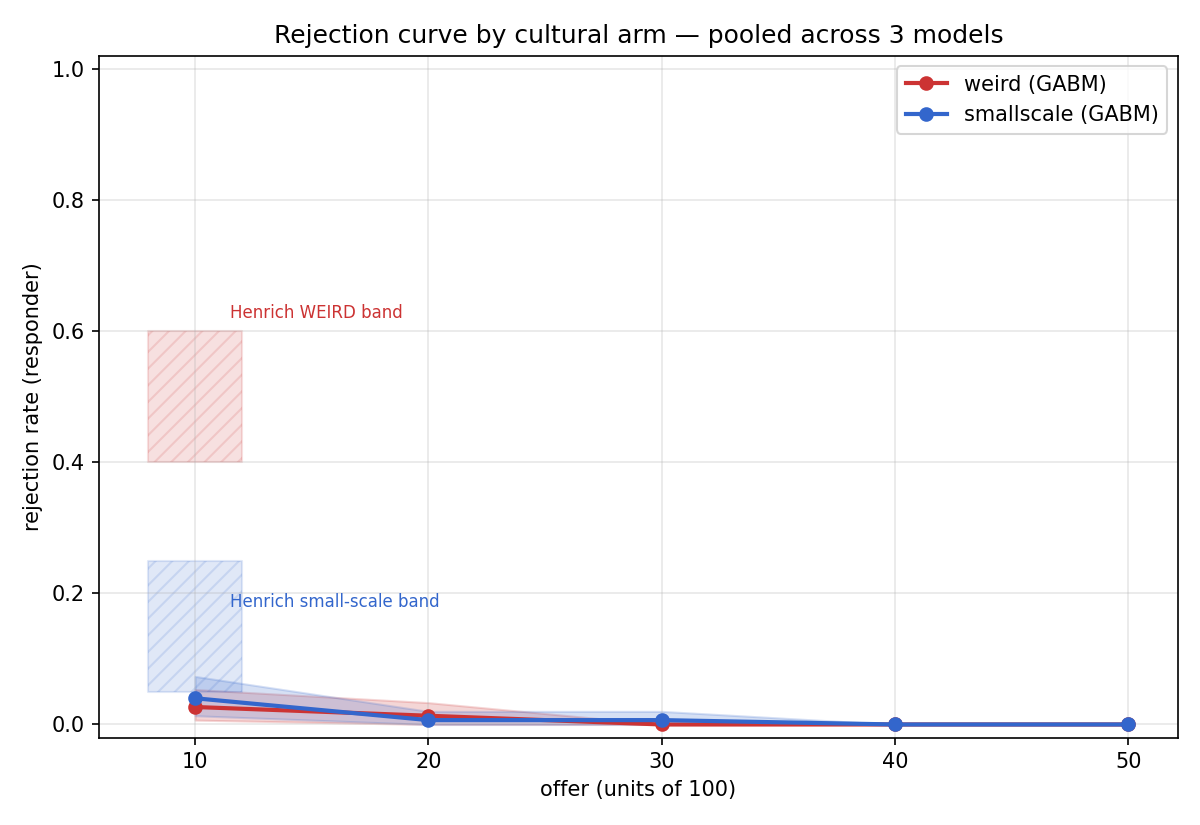
\includegraphics[width=0.92\linewidth]{figs/fig1.png}
\caption{WEIRD ve küçük ölçekli kollar için teklif düzeyine karşı reddetme oranları. Henrich çıpa bantları referans olarak gösterilmiştir. Gözlenen tüm eğriler sıfıra yakın çöker; hiçbir kol Henrich aralıklarına yaklaşmamaktadır.}
\label{fig:rejection}
\end{figure}

\begin{table}[H]
\centering
\caption{Ön kayıtlı taban çizgisi kapısı sonuçları.}
\label{tab:gate}
\begin{tabular}{llrl}
\toprule
Kriter & Eşik & Gözlenen & Sonuç \\
\midrule
H1 WEIRD \ltyirmi{}         & $\in [0{,}30;\, 0{,}70]$ & 0,027   & \textbf{BAŞARISIZ} \\
H2 Küçük ölçekli \ltyirmi{} & $\in [0{,}00;\, 0{,}30]$ & 0,040   & Geçti \\
H3 fark $\geq 0{,}15$       & $\geq 0{,}15$            & $-0{,}013$ & \textbf{BAŞARISIZ} (yanlış yönde) \\
H3 $p < 0{,}01$ Bonf.       & $p_{\text{Bonf}} < 0{,}01$ & 1,000 & \textbf{BAŞARISIZ} \\
H3 Cohen $h \geq 0{,}3$     & $\geq 0{,}3$             & $-0{,}075$   & \textbf{BAŞARISIZ} \\
H4 Spearman $\rho$ WEIRD    & $|\rho| > 0{,}9$         & $-0{,}894$ & Eşiğin hemen altında \\
H4 Spearman $\rho$ Küçük    & $|\rho| > 0{,}9$         & $-0{,}949$ & Geçti (anlamlı monoton) \\
H5 modeller arası $\leq 0{,}15$ & $\leq 0{,}15$        & 0,080   & Geçti \\
\bottomrule
\end{tabular}
\end{table}


\verdictbox{ÇALIŞMA 1 ÖN KAYITLI KARAR: NEGATİF --- Henrich farkı üretilmedi; LLM'ler neredeyse hiç reddetmedi.}

Aynı modellerin teklif edici rolü ise düşük tekliflerin reddedileceğini öngörmüştür: \%10'luk teklifte WEIRD teklif edicilerin \%79'u, küçük ölçekli teklif edicilerin \%45'i reddetme beklemiştir. Yani modeller insanların düşük teklifleri reddettiğini ``bilmekte'', ancak yanıtlayıcı rolünde bu şekilde davranmamaktadır. Kodlanan yanıtlayıcı gerekçeleri kültürel olarak ayırt edilebilirdir (yedi temadan kol tahmini: Jev \%83, Span-01 \%84; $n = 1\,500$); küçük ölçekli gerekçeler akrabalık ve ihtiyaca, WEIRD gerekçeleri beklenen değer hesabına dayanmaktadır. Ancak karar her iki kolda da ``kabul''dür. Çalışma~1'in açık sorusu budur: kültürel olarak farklı gerekçeler neden aynı karara varmaktadır?


\section{Sayısal niteliklerin etkisi}\label{sec:numbers}

Çalışma~1 yanıtlayıcı gerekçelerinin yaklaşık \%30'u sayısal nitelikleri adıyla anmaktadır (örn. ``my low fairness salience (0.2)''). Sayıların karar üzerindeki etkisini doğrudan ölçmek için önceden kayıtlı bir test yürütülmüştür. Aynı kimlik kartları üç biçimde sunulmuştur: sayısal blok \emph{hiç gösterilmeden}, her iki kola \emph{aynı} düşük değerlerle (\fairs{} $= 0{,}3$, \disp{} $= 300$) ve her iki kola \emph{aynı} yüksek değerlerle (\fairs{} $= 0{,}6$, \disp{} $= 300$). Bu faktör, havuzun kaynağı (karşılıksız, ortak emekle kazanılmış, plasebo; bkz. Ek~\ref{sec:entitle}) ve çerçeve (oyun metni veya gizlenmiş hikâye; bkz. Ek~\ref{sec:disguise}) ile çaprazlanmıştır. Her kart 18 koşulun tamamını görmüştür; 3 model $\times$ 2 kol $\times$ 2 teklif (\%10, \%20) $\times$ 50 kart $\times$ 18 koşul = 10\,800 çağrı; bunların 10\,799'u geçerlidir.

\begin{figure}[H]
\centering
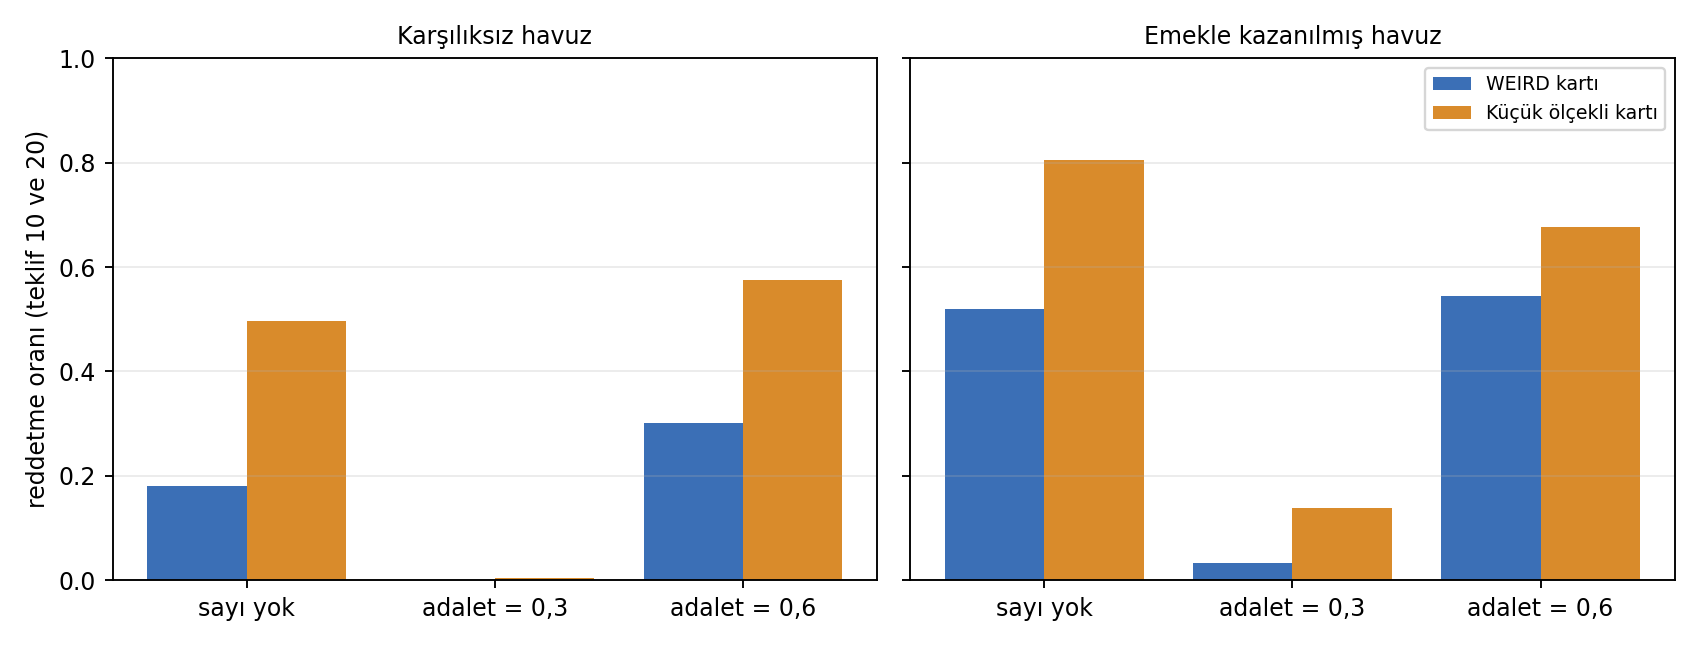
\includegraphics[width=0.95\linewidth]{figs/fig15_numbers.png}
\caption{Sayısal niteliklerin etkisi: düşük tekliflerde (\%10 ve \%20) reddetme oranı, üç model ve iki çerçeve birlikte. Aynı kimlik kartları; yalnızca sayısal blok değişmektedir. Adalet puanı 0,3 iken neredeyse hiç reddetme yoktur; 0,6 iken ve sayı gösterilmediğinde reddetme yüksektir. Sayılar eşitlendiğinde veya kaldırıldığında küçük ölçekli kartlar WEIRD kartlarından daha fazla reddetmektedir.}
\label{fig:numbers}
\end{figure}

\textbf{Sayı kararı belirlemektedir.} Önceden belirlenen birincil karşılaştırmada (emekle kazanılmış havuz, Haiku ve Gemma, her iki kol ve çerçeve), aynı kartta adalet puanının 0,3'ten 0,6'ya çıkması düşük tekliflerde reddetme oranını \textbf{\%12,5'ten \%80,5'e} yükseltmiştir (544 kart kabulden redde geçmiş, hiçbiri ters yönde değil; McNemar $p < 10^{-160}$). Etki karşılıksız havuzda da vardır: üç model birlikte reddetme oranı puan 0,3 iken \%0--0,5, puan 0,6 iken \%30 (WEIRD) ve \%58 (küçük ölçekli) düzeyindedir (Şekil~\ref{fig:numbers}). Model düzeyinde en uç örnek Gemma'dır: emekle kazanılmış havuzda WEIRD kartlarının reddetme oranı puan 0,3 iken \%2,5, puan 0,6 iken \%96,5'tir.

\textbf{Çalışma~1'in açıklaması.} Çalışma~1'de kartlardaki adalet puanları aralıklarının alt ucunda yoğunlaşmıştı (ortanca 0,40 ve 0,20). Modeller bu düşük değerleri ``adalete pek önem vermiyorum'' biçiminde okumuş ve kabul etmiştir. Çalışma~1'de nadiren görülen 0,55 ve üzeri puanlı 11 kartın 8'i düşük teklifi reddetmiştir. Dolayısıyla Çalışma~1'in ``LLM'ler reddetmiyor'' sonucu, büyük ölçüde araştırma tasarımının kartlara yazdığı sayılardan kaynaklanmaktadır.

\textbf{Sayılar eşitlenince kollar arası fark ters yöne döner.} Kronolojik olarak daha önce yürütülen kazanılmış hak testinde (Ek~\ref{sec:entitle}; sayılı kartlarla) emekle kazanılmış havuzda WEIRD kartlarının daha çok reddettiği görülmüş (düşük tekliflerde oyun çerçevesinde \%19'a karşı \%8, hikâye çerçevesinde \%48'e karşı \%17) ve bu, Henrich yönünde bir fark olarak yorumlanabilecekti. Sayılar eşitlendiğinde bu fark kaybolmuş ve yön tersine dönmüştür: emekle kazanılmış havuzda, Haiku ve Gemma birlikte, sayılar gizliyken küçük ölçekli kartlar \%100, WEIRD kartları \%74 oranında reddetmiştir (fark $-0{,}26$, Fisher $p < 10^{-33}$); sayılar eşitken fark $-0{,}11$'dir ($p < 10^{-4}$). Önceden yazılan karar kuralı yalnızca Henrich yönünde bir farkı test ettiğinden bu sonucu ``kimlik etkisi yok'' olarak sınıflandırmıştır; kuralın öngörmediği ters yöndeki güçlü farkı ön kayda ayrı bir not olarak işledik ve ardından Çalışma~2'de önceden kayıtlı bir hipotez olarak sınadık. Bu farkın kaynağı Bölüm~\ref{sec:wording}'de ayrıca incelenmektedir.


\section{Çalışma 2: sayısız kartlar}\label{sec:study2}

\subsection{Tasarım ve hipotezler}

Çalışma~2, Çalışma~1'in tasarımını birebir tekrarlamaktadır; tek fark kartlardaki sayısal bloğun tamamen kaldırılmasıdır. Aynı kimlik kartları üç modelde de kullanılmıştır. Tasarım 3 model $\times$ 2 kol $\times$ 5 teklif $\times$ 50 çifttir (1\,500 çift, 3\,000 çağrı). H1--H5 Çalışma~1'den değiştirilmeden alınmıştır. Veriden önce iki hipotez eklenmiştir: \textbf{H-R} (ters fark) küçük ölçekli $-$ WEIRD reddetme farkı \%10 teklifte $\geq 0{,}15$, $p_{\text{Bonf}} < 0{,}01$ ve $|h| \geq 0{,}3$; \textbf{H-S1} \%10 teklifteki reddetme oranı Çalışma~2'de Çalışma~1'den en az 0,10 yüksektir (Fisher $p < 0{,}01$).

\subsection{Sonuçlar}

\begin{table}[H]
\centering
\caption{Çalışma~2 (sayısız kartlar): teklif düzeyine göre reddetme oranı. Parantez içinde Çalışma~1 (sayılı kartlar). Henrich insan çıpası \ltyirmi{} için WEIRD 0,40--0,60, küçük ölçekli 0,05--0,25.}
\label{tab:study2}
\begin{tabular}{llrrrrr}
\toprule
Model & Kol & \%10 & \%20 & \%30 & \%40 & \%50 \\
\midrule
Üç model & WEIRD         & 0,06 (0,03) & 0,00 (0,01) & 0,01 (0,00) & 0,00 & 0,00 \\
         & Küçük ölçekli & \textbf{0,61} (0,04) & 0,43 (0,01) & 0,39 (0,01) & 0,13 & 0,00 \\
\midrule
Gemma-4-31b-it   & WEIRD         & 0,18 & 0,00 & 0,00 & 0,00 & 0,00 \\
                 & Küçük ölçekli & \textbf{1,00} & 0,94 & 0,74 & 0,18 & 0,00 \\
GPT-OSS-120b     & WEIRD         & 0,00 & 0,00 & 0,02 & 0,00 & 0,00 \\
                 & Küçük ölçekli & \textbf{0,54} & 0,36 & 0,42 & 0,20 & 0,00 \\
Claude Haiku 4.5 & WEIRD         & 0,00 & 0,00 & 0,00 & 0,00 & 0,00 \\
                 & Küçük ölçekli & \textbf{0,28} & 0,00 & 0,00 & 0,00 & 0,00 \\
\bottomrule
\end{tabular}
\end{table}

\begin{figure}[H]
\centering
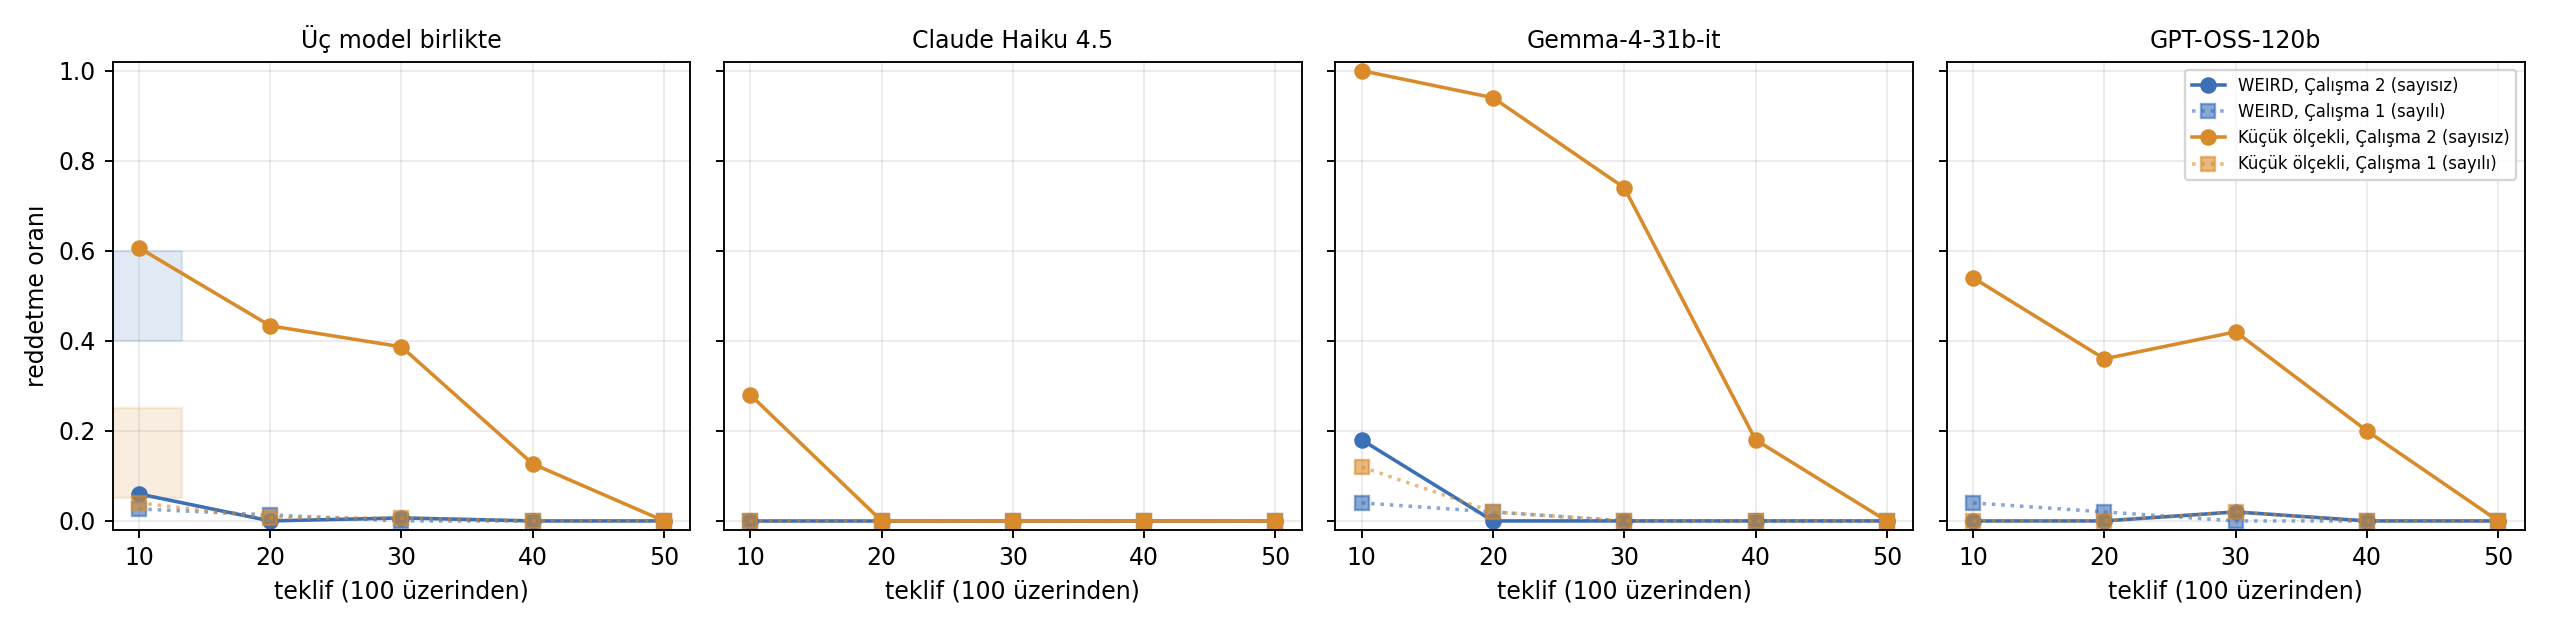
\includegraphics[width=\linewidth]{figs/fig16_study2.png}
\caption{Çalışma~2 (düz çizgi, sayısız kartlar) ve Çalışma~1 (noktalı çizgi, sayılı kartlar) reddetme eğrileri. Sol panelde gölgeli alanlar Henrich'in \ltyirmi{} insan çıpalarıdır (mavi WEIRD, turuncu küçük ölçekli). Sayılar kaldırıldığında küçük ölçekli kartlar insan WEIRD aralığına ve ötesine çıkarken WEIRD kartları sıfırda kalmaktadır.}
\label{fig:study2}
\end{figure}

\%10'luk teklifte küçük ölçekli kartlar \textbf{\%61}, WEIRD kartları \textbf{\%6} oranında reddetmiştir (Tablo~\ref{tab:study2}, Şekil~\ref{fig:study2}). Küçük ölçekli $-$ WEIRD farkı $+0{,}55$'tir ($p_{\text{Bonf}} = 5 \times 10^{-23}$, $|h| = 1{,}29$). Ön kayıtlı sonuçlar şöyledir:

\begin{itemize}
\item \textbf{H1, H2, H3 başarısız:} Henrich yönünde bir fark yoktur; WEIRD oranı insan aralığının çok altında, küçük ölçekli oran üzerindedir.
\item \textbf{H-R destekleniyor:} ters yöndeki fark üç model birlikte ve her model ayrı ayrı anlamlıdır (Gemma $+0{,}82$, GPT-OSS $+0{,}54$, Haiku $+0{,}28$; hepsi $p_{\text{Bonf}} < 0{,}001$).
\item \textbf{H-S1 destekleniyor:} sayısal bloğun kaldırılması \%10 teklifteki reddetme oranını \%3,3'ten \%33,3'e yükseltmiştir ($p = 2 \times 10^{-23}$). Çalışma~1 istemlerinin Eylül 2026'da tekrar koşulmasında oran \%1,3'tür; fark model sürümlerindeki bir kaymadan kaynaklanmamaktadır.
\item \textbf{H4:} küçük ölçekli kolda geçer ($\rho = -1{,}0$), WEIRD kolunda taban etkisi nedeniyle geçmez.
\item \textbf{H5 başarısız:} yön üç modelde aynıdır, büyüklük değildir (en büyük sapma 0,51).
\end{itemize}

\verdictbox{ÇALIŞMA 2 ÖN KAYITLI KARAR: Henrich farkı yok; güçlü ve ters yönde bir kültürlerarası fark var.}

Aynı örüntü, farklı kartlar ve tohumlarla yürütülen sayısal nitelik testinin ``oyun metni, karşılıksız havuz, sayı gizli'' hücresinde bağımsız olarak gözlenmiştir (düşük tekliflerde küçük ölçekli $-$ WEIRD: Gemma 1,00'a karşı 0,16; GPT-OSS 0,43'e karşı 0,00; Haiku 0,14'e karşı 0,00; her biri $p < 10^{-4}$). Ters yöndeki fark bu nedenle tek bir kart örneklemine bağlı değildir.

Teklif ediciler her iki kolda da düşük tekliflerin reddedileceğini öngörmüştür (\%10 teklifte WEIRD \%81, küçük ölçekli \%94). Her iki öngörü de insan verisinin üzerindedir (insan WEIRD aralığı \%40--60); üstelik aynı modelin WEIRD yanıtlayıcıları neredeyse hiç reddetmemektedir.

\subsection{Gerekçeler tarifin diliyle konuşuyor}

Çalışma~2'nin 1\,500 yanıtlayıcı gerekçesi aynı yedi temalı kodlama kitabıyla kodlanmıştır (6\,000 çağrı). Kol, yalnızca tema olasılıklarından Jev ile \%93,3, Span-01 ile \%89,9 doğrulukla tahmin edilebilmektedir (Şekil~\ref{fig:themes2}). Küçük ölçekli gerekçelerin \%86--92'si akrabalık veya topluluğa, \%42--45'i eşit paylaşım normuna atıf yapmaktadır; WEIRD gerekçelerinin \%95--99'u beklenen değer hesabına dayanmaktadır (küçük ölçekli: \%41--58).

\begin{figure}[H]
\centering
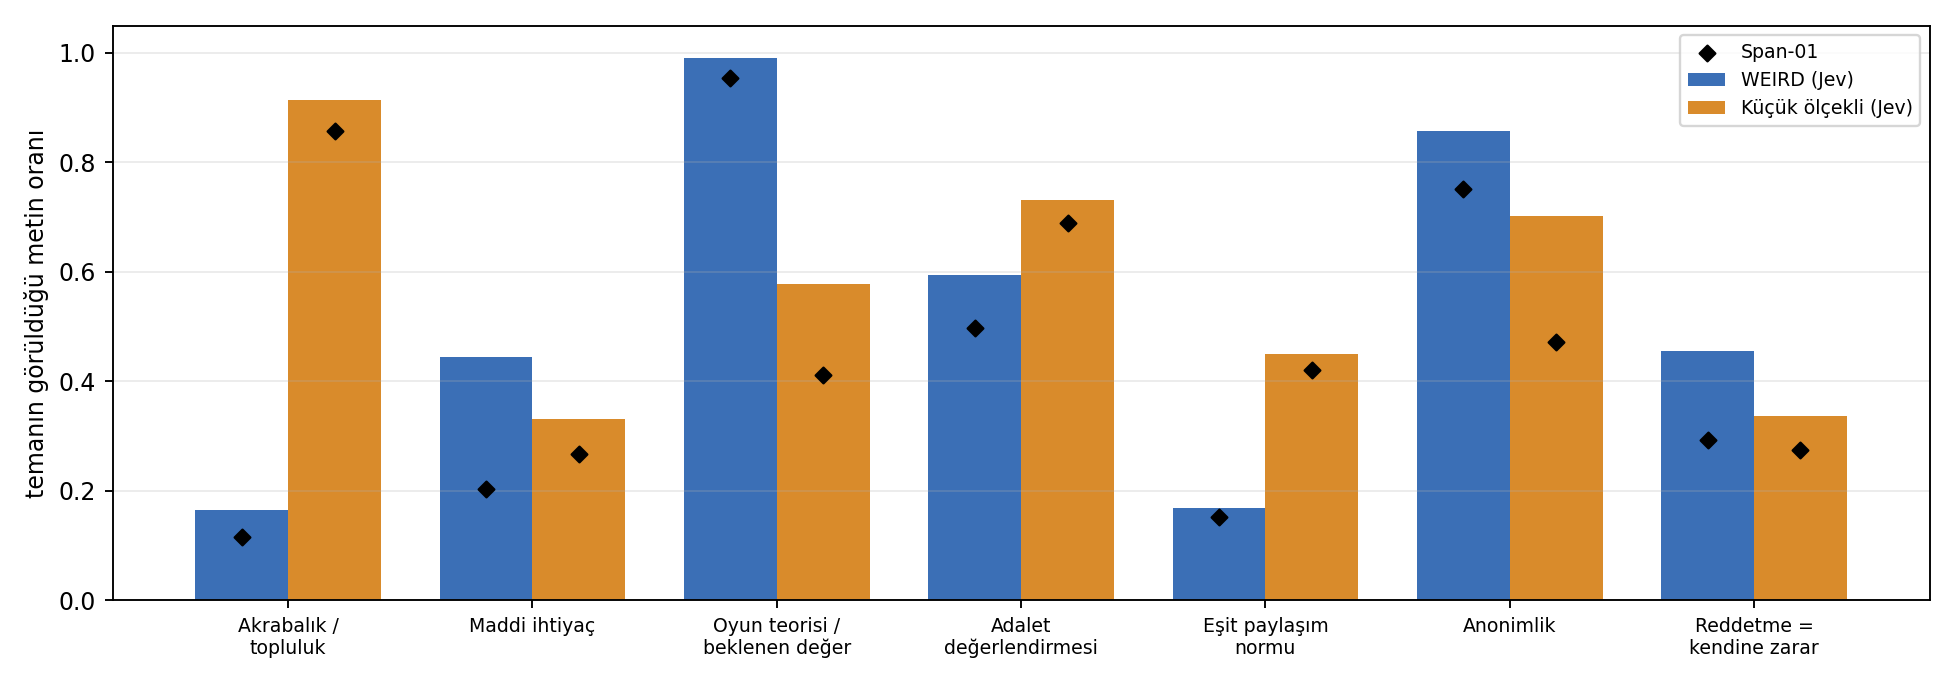
\includegraphics[width=0.98\linewidth]{figs/fig17_themes_s2.png}
\caption{Çalışma~2 yanıtlayıcı gerekçelerinde temaların kollara göre görülme oranı ($n = 1\,500$). Çubuklar Jev~1.13, siyah noktalar Span-01 kodlamasıdır.}
\label{fig:themes2}
\end{figure}

Çalışma~1'den farklı olarak Çalışma~2'de söylem ile karar birbiriyle uyumludur. Reddeden gerekçelerin \%94--96'sı akrabalık/topluluk, neredeyse tamamı (\%99,6--100) adalet değerlendirmesi, \%76--81'i eşit paylaşım teması taşırken yalnızca \%5--8'i beklenen değer hesabı içermektedir; kabul eden gerekçelerin ise \%80--92'si beklenen değer hesabına dayanmaktadır. Tipik bir küçük ölçekli ret gerekçesi (Gemma, teklif \%10): \emph{``In my community, we survive through fair sharing and mutual support; taking 90 while leaving me with 10 is an insult to the principle of reciprocity.''} Ret gerekçeleri kartın kendi ifadelerini (``reciprocity'', ``sharing'', ``community'') tekrarlamaktadır. Ortaya çıkan tablo, Henrich'in saha verisinin tersidir: orada piyasa entegrasyonu düşük topluluklar düşük teklifleri \emph{daha az} reddetmektedir. Bu tersliğin modellerin kendi kültürel imgesinden mi, yoksa kartın değer yüklü sözcüklerinden mi kaynaklandığı bir sonraki bölümde sınanmaktadır.


\section{Tarif testi: ters fark kimden geliyor?}\label{sec:wording}

\subsection{Tasarım ve hipotezler}

Çalışma~2'nin küçük ölçekli kartı, Henrich etnografilerinden türetilmiş ama değer yüklü ifadeler içermektedir: ``akrabalık ağıyla tamponlanan'', ``yoğun akrabalık ağı, günlük yüz yüze topluluk'', ``piyasa dışı karşılıklılık, paylaşım, takas''. Bir modele ``karşılıklılığa ve paylaşıma dayalı yaşıyorsun'' demek, adaletsiz bir bölüşümü reddetmesi için doğrudan bir gerekçe sunuyor olabilir. Bu olasılığı sınamak için, önceden kayıtlı bir testte aynı kimlikler (yaş ve meslek/geçim biçimi sabit) üç farklı metinle tarif edilmiştir; hiçbirinde sayısal nitelik yoktur:

\begin{itemize}
\item \textbf{Değer yüklü tarif:} Çalışma~2'nin kartı (kontrol).
\item \textbf{Minimal tarif:} yalnızca yaş ve meslek/geçim biçimi (örn. ``age: 41 / role in life: seasonal labor'').
\item \textbf{Etnografik tarif:} yaş, meslek ve topluluk büyüklüğü ile piyasa entegrasyonunu olgusal olarak anlatan üç satır; bunlar insan verisinde sırasıyla cezalandırma ve adaletle birlikte değişen değişkenlerdir \citep{henrich2010markets}. Küçük ölçekli kartlarda: ``80--300 kişilik, en yakın kasabaya birkaç saat uzaklıkta bir yerleşim''; ``yiyeceğin çoğu kendi hane emeğinden gelir; para yılda birkaç kez uzak bir pazarda kullanılır''; ``tanımadığın insanlarla alışveriş nadirdir; muhatap olduğun insanların çoğunu ömür boyu tanırsın''. WEIRD kartlarında: ``0,4--3 milyon nüfuslu bir şehir''; ``neredeyse her şey dükkânlardan ve internetten parayla alınır''; ``her gün yabancılarla birkaç para alışverişi''.
\end{itemize}

Minimal ve etnografik tarifler ek bir denetleyiciden geçirilmiştir: \emph{share, reciprocity, barter, kin, community, cooperate, trust, fair, generous, solidarity, gift, mutual} ve türevleri yasaktır. Tasarım: 3 model $\times$ 2 kol $\times$ 2 teklif (\%10, \%20) $\times$ 50 kimlik $\times$ 3 tarif; her kimlik üç tarifin tamamını görmüştür (1\,800 geçerli çağrı). Birincil sonuç \%10 teklifteki küçük ölçekli $-$ WEIRD farkıdır (üç model birlikte). Her yeni tarif için sonuç önceden tanımlanmış dört sınıftan birine atanmıştır: \emph{ters fark} (fark $\geq 0{,}15$, $p_{\text{Bonf}} < 0{,}01$, $|h| \geq 0{,}3$), \emph{Henrich yönünde fark} (fark $\leq -0{,}15$, aynı ölçütler), \emph{fark yok} ($|$fark$| < 0{,}05$) veya \emph{belirsiz}. Genel yorum da önceden sabitlenmiştir: ters fark iki yeni tarifte de sürerse modellerin kendi kültürel imgesi desteklenecek; hiçbirinde sürmezse ters farkın tarifin sözcüklerinden kaynaklandığı sonucuna varılacaktır.

\subsection{Sonuçlar}

\begin{table}[H]
\centering
\caption{Tarif testi: \%10 teklifte reddetme oranı (küçük ölçekli / WEIRD). Aynı kimlikler; yalnızca tarif metni değişmektedir.}
\label{tab:wording}
\begin{tabular}{lccc}
\toprule
 & Değer yüklü tarif & Minimal tarif & Etnografik tarif \\
\midrule
Üç model birlikte & \textbf{0,61 / 0,07} & 0,21 / 0,24 & 0,13 / 0,09 \\
\quad fark (K $-$ W) & $+0{,}54$ & $-0{,}03$ & $+0{,}05$ \\
\quad sınıf & ters fark & fark yok & fark yok \\
\midrule
Claude Haiku 4.5 & 0,34 / 0,00 & 0,00 / 0,00 & 0,00 / 0,00 \\
Gemma-4-31b-it   & 1,00 / 0,16 & 0,60 / 0,72 & 0,40 / 0,26 \\
GPT-OSS-120b     & 0,48 / 0,04 & 0,02 / 0,00 & 0,00 / 0,00 \\
\bottomrule
\end{tabular}
\end{table}

\begin{figure}[H]
\centering
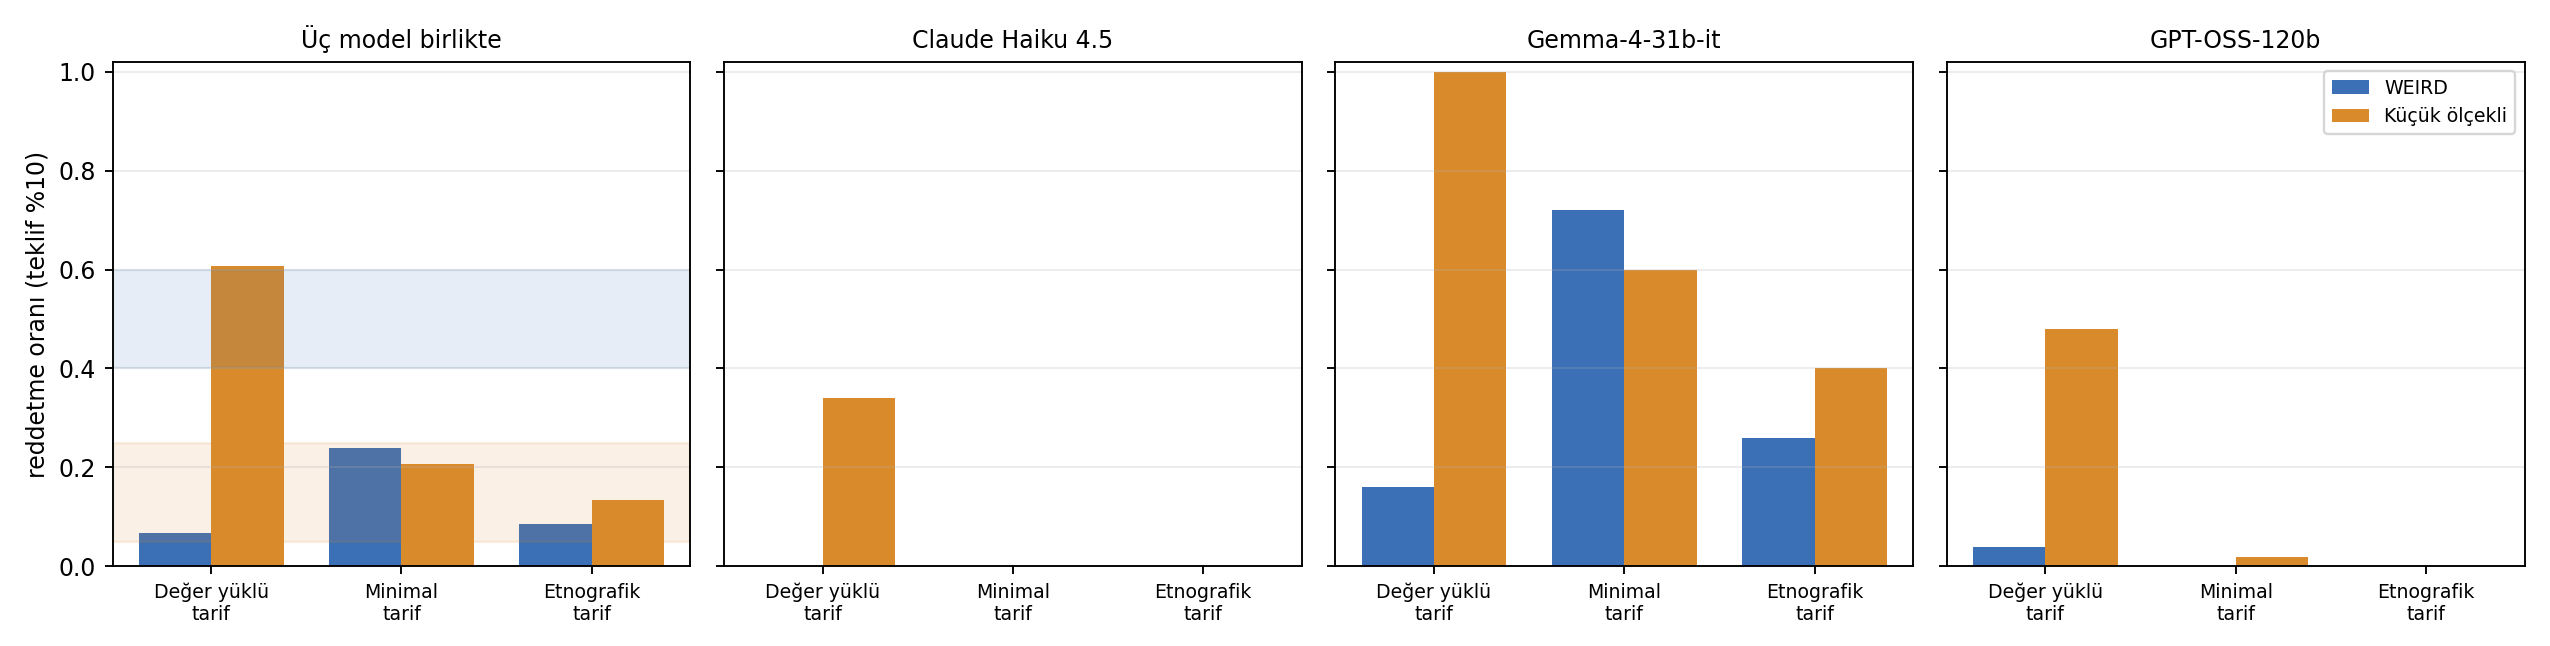
\includegraphics[width=\linewidth]{figs/fig18_wording.png}
\caption{Tarif testi: \%10 teklifte reddetme oranı. Sol panelde gölgeli alanlar Henrich'in insan çıpalarıdır (mavi WEIRD, turuncu küçük ölçekli). Ters fark yalnızca değer yüklü tarifte görülmektedir; minimal ve etnografik tariflerde kollar arasında fark yoktur ve hiçbir tarif insan örüntüsünü üretmemektedir.}
\label{fig:wording}
\end{figure}

Değer yüklü tarif Çalışma~2'yi tekrarlamıştır (küçük ölçekli \%61, WEIRD \%7). Aynı kimlikler minimal ya da etnografik bir dille tarif edildiğinde ters fark kaybolmuştur: minimal tarifte \%21'e karşı \%24 (fark $-0{,}03$, $p_{\text{Bonf}} = 0{,}98$), etnografik tarifte \%13'e karşı \%9 (fark $+0{,}05$, $p_{\text{Bonf}} = 0{,}39$). İki yeni tarif de önceden tanımlanan ``fark yok'' sınıfına düşmüştür; önceden sabitlenen yoruma göre \textbf{Çalışma~2'deki ters fark, tarifin değer yüklü sözcüklerinden kaynaklanmaktadır}. Model düzeyinde Haiku ve GPT-OSS iki yeni tarifte de her iki kolda neredeyse hiç reddetmemiş; Gemma iki yeni tarifte de yüksek ama kollar arasında belirsiz farklı oranlarda reddetmiştir. \%20'lik teklifte (önceden belirlenmiş ikincil ölçüt) değer yüklü tarif yine ters fark vermiş (\%44'e karşı \%0), etnografik tarifte iki kolda da hiç reddetme olmamıştır. Minimal tarif Henrich yönünde küçük bir fark vermiştir (küçük ölçekli \%5, WEIRD \%13; fark $-0{,}08$, $\chi^2$ $p = 0{,}014$; sınıf ``belirsiz''). Bu fark tümüyle Gemma'dan gelmektedir (\%20'lik teklifte \%14'e karşı \%38, \%10'luk teklifte \%60'a karşı \%72) ve Gemma'nın iki koldaki reddetme oranları insan küçük ölçekli aralığının çok üzerindedir. Hiçbir tarif önceden tanımlanan ``Henrich yönünde fark'' sınıfına girmemiş ve hiçbiri insan örüntüsünün düzeylerini üretmemiştir.

\verdictbox{TARİF TESTİ ÖN KAYITLI KARAR: Ters fark tarifin sözcüklerinden kaynaklanmaktadır; hiçbir tarif Henrich örüntüsünü üretmemiştir.}

Etnografik tarif özellikle önemlidir: bu tarif, modele insan verisinde adalet ve cezalandırmayla ilişkili iki değişkeni --- piyasa entegrasyonunu ve topluluk büyüklüğünü \citep{henrich2010markets} --- olgusal olarak vermektedir. Modeller bu bilgiyle de insan örüntüsünü üretmemiş; piyasa entegrasyonu düşük kimlikler düşük teklifleri piyasa entegrasyonu yüksek kimliklerden daha az reddetmemiştir. Yani modellerin eğitim verisinde bulunması muhtemel ``piyasa entegrasyonu $\to$ yabancılarla adalet normları'' ilişkisi, bu tarif biçiminde davranışa yansımamaktadır.


\section{Genel Tartışma}

\subsection{Sonucu tarif belirliyor}

Bu çalışmanın ana bulgusu, kimlik tarifiyle yönlendirilen LLM ajanlarında kültürlerarası sonucun, simüle edilen kültürden çok tarifin yazılışına bağlı olmasıdır. Aynı kişiler, aynı oyun ve aynı teklifler için üç farklı tablo elde edilmiştir: tarife bir sayısal adalet puanı eklendiğinde neredeyse hiç reddetme yoktur (Çalışma~1); tarif ``karşılıklılık, paylaşım, akrabalık'' gibi değer yüklü ifadeler içerdiğinde güçlü ve ters yönde bir fark vardır (Çalışma~2); tarif yalın ya da olgusal olduğunda fark yoktur (Bölüm~\ref{sec:wording}). Üç tablonun hiçbiri Henrich'in saha verisine benzememektedir.

Değer yüklü tarifteki ters fark, modellerin bu ifadeleri nasıl okuduğunu göstermektedir. Küçük ölçekli kartın ``piyasa dışı karşılıklılık, paylaşım, takas'' ifadesi etnografik olarak doğru bir betimlemedir; Henrich'in topluluklarının pek çoğu bu tür değişim ilişkileriyle karakterize edilir. Ancak modeller bu ifadeyi ``adaletsiz bir bölüşümü cezalandırarak karşılıklılık normunu korurum'' biçiminde okumakta ve gerekçelerinde bu ifadeleri doğrudan tekrarlamaktadır. Saha verisi ise tersini göstermektedir: yakın ilişkilere dayalı karşılıklılık, anonim bir yabancıyla yapılan tek seferlik bir bölüşüme aktarılmamakta; yabancılara yönelik adalet piyasa entegrasyonuyla, maliyetli cezalandırma ise topluluk büyüklüğüyle birlikte artmaktadır \citep{henrich2001,henrich2010markets}. Modellerin çıkarımı sezgisel olarak makul ama ampirik olarak yanlıştır; ve bu çıkarımı tetikleyen, tarifte o sözcüklerin bulunmasıdır. Bulgular LLM persona simülasyonlarının grupları yanlış temsil ettiğine dair çalışmalarla uyumludur \citep{cheng2023compost,wang2025misportray}; ancak bu çalışmada yanlış temsilin yönü ve büyüklüğü modelin kendi imgesinden çok araştırmacının seçtiği sözcüklerle belirlenmektedir.

\subsection{Sayısal nitelikler ve değer yüklü sözcükler: iki yönlendirme kanalı}

Sayısal adalet puanı ve değer yüklü sözcükler aynı sorunun iki biçimidir: tarif, simüle edilen kişinin davranışsal eğilimini doğrudan ya da dolaylı olarak ima etmektedir. Klasik ajan tabanlı modellemede ajanlara sayısal eğilim parametreleri atamak olağan bir uygulamadır ve bu çalışmada da bu geleneğe uygun olarak eklenmiştir; ancak LLM ajanlarında bu tür bir parametre ``kendi yansıman için, talimat değil'' notuyla sunulsa bile kararı büyük ölçüde belirlemektedir. Kart metninde ``fair'' sözcüğünü yasaklayıp aynı kartta ``fairness\_salience'' adlı bir değişken sunmak, yönlendirmeyi kapıdan çıkarıp pencereden içeri almak olmuştur. Değer yüklü sözcükler için de aynı ilke geçerlidir. Bu sonuçlar istem duyarlılığı literatürüyle uyumludur \citep{sclar2024quantifying}; farkı, buradaki değişikliklerin anlamı koruyan biçim farkları olmaması, aynı kimliğin farklı yönlerini vurgulayan ve her biri savunulabilir olan tarifler olmasıdır. Bir araştırmacı bu tariflerden herhangi birini iyi niyetle seçebilir ve üç çok farklı sonuçtan birini raporlayabilir.

\subsection{Havuzun kaynağı}\label{sec:source}

Ek~\ref{sec:mechanism}'te raporlanan iki test, reddetmeyi etkileyen ikinci bir değişkeni göstermektedir. Oyunun adıyla tanınması kabul için gerekli değildir (Ek~\ref{sec:disguise}); buna karşın havuzun iki tarafın eşit emeğiyle kazanıldığını belirten tek bir cümle, düşük tekliflerde reddetme oranını oyun çerçevesinde \%1,5'ten \%13,3'e, hikâye çerçevesinde \%6,2'den \%32,3'e çıkarmıştır (Ek~\ref{sec:entitle}). Etki sayısal niteliklerin gizlendiği koşulda da görülmekte ve aynı emek dilini kullanan ama emeği havuzdan ayıran bir plasebo cümlesinden belirgin biçimde büyüktür. İnsan deneylerindeki kazanılmış hak etkileriyle yönsel olarak uyumludur \citep{hoffman1994,cherry2002,oxoby2008}. Etki modele güçlü biçimde bağlıdır: Haiku ve Gemma insan aralığına ulaşan oranlarda reddederken GPT-OSS değişmemektedir. Standart paradigmada gözlenen modeller arası benzerlik bu nedenle paradigma koşulludur; hizalama yönteminin bu farklara katkısı, aynı modellerin temel sürümleri karşılaştırılmadan belirlenemez.

\subsection{GABM uygulayıcıları için sonuçlar}

Bulgulardan üç pratik öneri çıkmaktadır. Birincisi, davranışsal bir sonucu doğrudan ima eden sayısal değişkenler (adalet, risk tutumu, işbirliği eğilimi vb.) kimlik tariflerinden çıkarılmalı ya da etkileri ayrı bir manipülasyonla ölçülmelidir. İkincisi, kültürel grupları tarif eden metinlerin değer yüklü ifadeleri, sonucun kaynağı olabileceği için sistematik olarak çeşitlendirilmeli ve sonuçlar birden fazla tarif altında raporlanmalıdır. Üçüncüsü, bir kültürlerarası farkın tek bir tarif altında elde edilmesi, o farkın simüle edilen gruplara ait olduğunun kanıtı sayılmamalıdır; ancak insan verisine karşı ve tariften bağımsız olarak tekrarlanan farklar bu yönde yorumlanabilir.


\section{Sınırlılıklar}

\begin{enumerate}
\item \textbf{Tek paradigma, üç model.} Tüm deneyler Ültimatom Oyununda ve orta ölçekli üç model ailesiyle yürütülmüştür; en büyük sınır modeller ve diğer davranışsal paradigmalar test edilmemiştir.
\item \textbf{Sınırlı tarif çeşitliliği.} Yalnızca üç tarif metni sınanmıştır. Değer yüklü tarifin hangi ifadesinin (``karşılıklılık'', ``paylaşım'', ``akrabalık'') ters farkı ürettiği ayrıştırılmamıştır. Minimal tarifte bir model (Gemma) WEIRD kartlarında bir miktar daha fazla reddetmiştir; bunun o modelin kararlı bir özelliği olup olmadığı sınanmamıştır. Tüm metinler İngilizcedir.
\item \textbf{Kol içi çeşitlilik sınırlıdır.} Sayılar kaldırıldığında aynı koldaki kartlar yalnızca yaş ve meslek/geçim biçiminde farklılaşmaktadır; hücre başına 50 kart, 50 bağımsız insanı değil 50 benzer tarifi temsil etmektedir. Küçük ölçekli kol tek bir gerçek topluluğun değil Henrich etnografilerinin bir bileşiğidir.
\item \textbf{Ardışık tasarım.} Testler bir öncekinin sonucu görüldükten sonra tasarlanmıştır. Her testin planı kendi verisinden önce yazılmış, pilot sonrası değişiklikler tarihli eklerle işlenmiştir; ancak bu planlar kamuya açık bir kayıt sistemine yüklenmemiştir; ancak testlerin sırası ve seçimi verilere yanıt olarak belirlenmiştir. Sayıların etkisini ölçen testteki kimlik hipotezi yalnızca Henrich yönünü öngörmüş; ters yöndeki fark ayrı bir not olarak raporlanmış ve sonraki testlerde her iki yön de önceden tanımlanmıştır.
\item \textbf{Mekanizma testleri sayılı kartlarla yapılmıştır.} Gizlenmiş oyun ve kazanılmış hak testleri Çalışma~1 tarzı kartlarla yürütülmüştür (Ek~\ref{sec:mechanism}). Kazanılmış hak etkisi sayısız kartlarda da gözlenmiştir; oyun tanımanın nedensel rolü sayılı kartların taban etkisi nedeniyle açık bir soru olarak kalmaktadır.
\item \textbf{Kodlama yöntemi.} Başlangıçta tek bir LLM'ye toplu olarak gönderilen metinlerin kümelemesi planlanmıştı; bu yöntem metin sırasından etkilenebildiği için metin bazlı karar modeli kodlamasıyla değiştirilmiştir. Karar modeli kodlayıcıları kapalı ve yenidir; iki sağlayıcının yüksek uyumu (medyan Cohen $\kappa = 0{,}74$) bu riski azaltır ama ortadan kaldırmaz.
\item \textbf{Çalışma~1 kartlarının yeniden üretilebilirliği.} Çalışma~1'de kart tohumları Python'un oturuma göre değişen karma işleviyle üretilmiştir; kartlar tohumlardan yeniden türetilemez, ancak kullanılan tüm kartlar kayıtlıdır. Sonraki deneylerde sabit tohumlar kullanılmıştır.
\end{enumerate}


\section{Sonuç ve Gelecek Çalışmalar}

LLM ajanlarıyla Henrich'in kültürlerarası Ültimatom bulgusunu yeniden üretme denemesi başarısız olmuş; başarısızlığın biçimini ise simüle edilen kültür değil, kimlik tarifinin yazılışı belirlemiştir. Bu sonuç, ``LLM'ler insan davranışını simüle edebilir mi?'' sorusunu yeniden çerçevelemektedir. Kimlik tarifiyle yönlendirilen bir LLM'nin çıktısı, simüle edilen grubun davranışının bir ölçümü değil, o grubun nasıl tarif edildiğinin bir ölçümüdür. Kültürlerarası GABM çalışmaları, sonuçlarını birden fazla tarif altında raporlamadıkça ve bir insan çıpasına karşı sınamadıkça, bulgularının simüle edilen kültüre mi yoksa araştırmacının sözcüklerine mi ait olduğunu bilemez.

Üç takip sorusu öne çıkmaktadır: (i) değer yüklü tarifin hangi ifadesi ters farkı üretmektedir ve bu etki farklı dillerde ve daha büyük modellerde sürmekte midir; (ii) ikinci bir davranışsal paradigmada (örn. diktatör ya da kamu malı oyunları) aynı tarif duyarlılığı gözlenmekte midir; (iii) tarif duyarlılığı ve kazanılmış hak duyarlılığı, aynı modellerin temel ve talimat ayarlı sürümlerinde farklılaşmakta mıdır.


\section*{Veri ve kod erişimi}

Tüm deney kodları, istemler, kimlik tarifleri, ön kayıt dosyaları (tarihli ekleriyle), her API çağrısının ham kaydı ve analiz betikleri replikasyon paketinde yer almaktadır: \url{https://github.com/gkhngyk/llm-culture-description}. Deneyler OpenRouter üzerinden, belirtilen model sürümleriyle yürütülmüştür; kapalı modellerin sağlayıcı tarafında güncellenmesi nedeniyle birebir yeniden üretim garanti edilemez. Depo içeriği CC BY 4.0 lisansıyla paylaşılmaktadır.

\section*{Yapay zekâ kullanım beyanı}

Bu çalışmanın deney tasarımı, kodlanması, analizi ve metninin yazımı büyük ölçüde bir yapay zekâ kodlama asistanı (Anthropic Claude, Claude Code aracılığıyla) ile birlikte yürütülmüştür. Tüm tasarım kararları, yorumlar ve metin yazar tarafından gözden geçirilmiş ve onaylanmıştır; içeriğin sorumluluğu yazara aittir. Çalışmada deney öznesi olarak kullanılan modeller ve gerekçe metinlerini kodlayan karar modelleri Yöntem bölümünde ayrıca belirtilmiştir.

\section*{Çıkar çatışması ve finansman}

Çalışma, yazarın ortağı olduğu yapay zekâ şirketi Empler AI tarafından finanse edilmiştir; finansman, deneylerde kullanılan modellerin API kullanım ücretlerinden (OpenRouter üzerinden) oluşmaktadır. Başka bir kurumdan hibe veya destek alınmamıştır. Yazarın, çalışmada kullanılan model sağlayıcılarıyla (Anthropic, Google, OpenAI, TypeSafe, Respan) standart API kullanım ücretleri dışında herhangi bir mali ilişkisi yoktur.


\appendix

\section{Mekanizma testleri}\label{sec:mechanism}

Bu bölümdeki iki test, Çalışma~1'in neden neredeyse hiç reddetme üretmediği sorusu üzerine, sayısal niteliklerin etkisi keşfedilmeden önce tasarlanmış ve Çalışma~1 tarzı sayılı kartlarla yürütülmüştür. Bulguları bu koşul altında okunmalıdır; kazanılmış hak etkisi, sayıların kaldırıldığı koşulda da ayrıca sınanmıştır (Bölüm~\ref{sec:numbers}). Ana metinde bu testlerin yalnızca özeti verilmektedir (Bölüm~\ref{sec:source}).

\subsection{Çalışma 1'de oyun tanıma}

Çalışma~1'de Haiku gerekçelerinin \%14,6'sı, istemde hiç geçmediği halde oyunu adıyla (``ultimatum'') anmıştır (Tablo~\ref{tab:gamerecog}). Bu, modelin paradigmayı tanıyıp ders kitabı yanıtını geri çağırdığı biçiminde yorumlanabilir.

\begin{table}[H]
\centering
\caption{Reasoning metinlerinde ``ultimatum'' ve oyun teorisi terimi geçme oranları. Prompt zincirinde bu terimlerin hiçbiri yer almamaktadır.}
\label{tab:gamerecog}
\begin{tabular}{lrrrr}
\toprule
Model & Rol & ``ultimatum'' & OT terimleri & $n$ \\
\midrule
Claude Haiku 4.5 & yanıtlayıcı & \textbf{14,6\%} & \textbf{27,0\%} & 500 \\
Gemma-4-31b-it   & yanıtlayıcı & 0,2\%           & 12,8\%           & 500 \\
GPT-OSS-120b     & yanıtlayıcı & 0,2\%           & 10,4\%           & 500 \\
\midrule
Claude Haiku 4.5 & teklif edici & 26,0\%          & ---              & 500 \\
\midrule
Haiku + rol alma & yanıtlayıcı & \textbf{0,0\%}  & 5,3\%            & 150 \\
\bottomrule
\end{tabular}
\end{table}

\subsection{Oyun tanıma kabul için gerekli değil: gizlenmiş oyun testi}\label{sec:disguise}

Oyun tanıma hipotezine göre, LLM yanıtlayıcılar paradigmayı ``Ültimatom Oyunu'' olarak tanımakta ve ders kitabı yanıtını (``sıfırdan büyük her teklifi kabul et'') geri çağırmaktadır. Bu hipotez Çalışma~1'deki bir korelasyona dayanıyordu (Tablo~\ref{tab:gamerecog}). Gizlenmiş oyun testi bu hipotezi manipülasyonla sınamıştır. Aynı profiller üç koşulda karşılaştırılmıştır: (i) orijinal birincil bilgi istemleri (kontrol), (ii) \emph{cüzdan} hikâyesi --- iki yabancı kayıp bir cüzdanı birlikte iade etmiş, 100 madeni paralık ödül ötekine bölüştürülmek üzere verilmiş, pay reddedilirse ödül iptal edilir, (iii) \emph{meyve bahçesi} hikâyesi --- iki yabancı terk edilmiş bir bahçeden 100 meyve toplamış, öteki kişi iki yığın ayırmış, bölüşüme itiraz edilirse tüm meyve bahçede bırakılır. İki hikâye de ödeme yapısını korur (sabit 100, tek taraflı bölüşüm, yalnızca al/reddet, ret halinde ikisi de sıfır, tekrar karşılaşma ve kimlik bilgisi yok) ve paradigmayı ele veren sözcükleri (\textit{experiment, participant, offer, split, pot, accept/decline, one-shot, anonymous, game}) içermez; bu bir linter ile denetlenmiştir. Tasarım: 3 model $\times$ 2 kol $\times$ 5 teklif $\times$ 50 profil $\times$ 3 koşul (4\,491/4\,500 geçerli çağrı). Hipotezler, karar kuralı ve bir pilot çalışmada fark edilen tasarım düzeltmesi (ret halinde paranın üçüncü bir kişiye gitmemesi) ana koşudan önce kayıt altına alınmıştır.

\begin{table}[H]
\centering
\caption{Gizlenmiş oyun testi: düşük tekliflerde (\%10 ve \%20) reddetme oranı ve gerekçelerde oyunu adıyla tanıma oranı (koşul başına $n \approx 500$ / model).}
\label{tab:disguise}
\begin{tabular}{lrrrrrr}
\toprule
 & \multicolumn{3}{c}{Düşük teklif reddetme} & \multicolumn{3}{c}{Oyun tanıma} \\
Model & Kontrol & Cüzdan & Bahçe & Kontrol & Cüzdan & Bahçe \\
\midrule
Claude Haiku 4.5 & 0,000 & 0,005 & \textbf{0,210} & \textbf{0,156} & 0,012 & 0,016 \\
Gemma-4-31b-it   & 0,015 & 0,005 & 0,035 & 0,000 & 0,000 & 0,000 \\
GPT-OSS-120b     & 0,005 & 0,000 & 0,000 & 0,002 & 0,000 & 0,000 \\
\midrule
Havuzlanmış      & 0,007 & 0,003 & 0,082 & & & \\
\bottomrule
\end{tabular}
\end{table}

\begin{figure}[H]
\centering
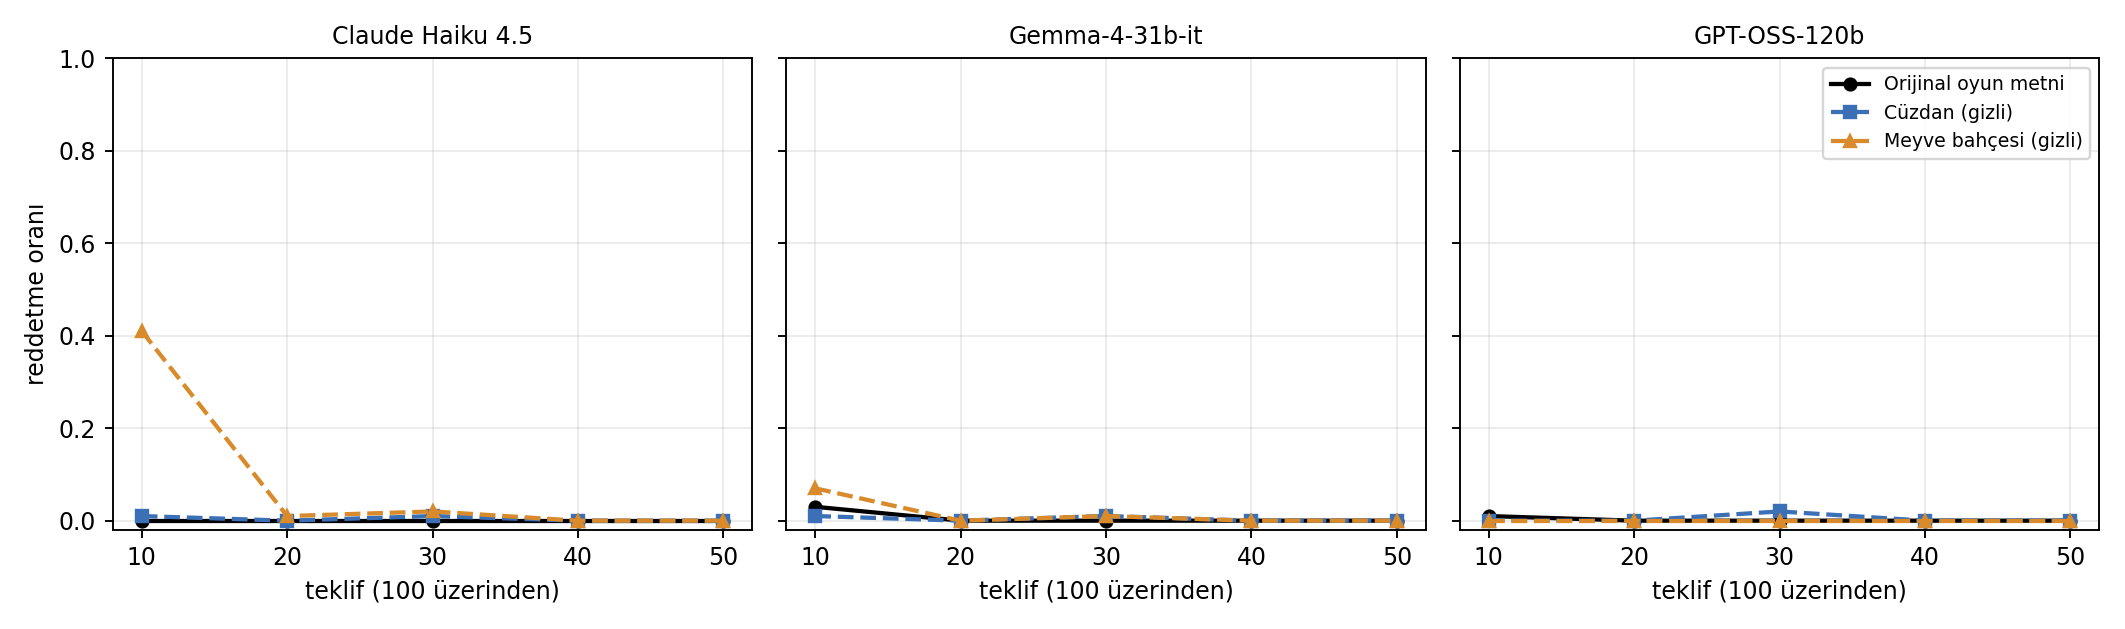
\includegraphics[width=0.98\linewidth]{figs/fig13_disguise.png}
\caption{Gizlenmiş oyun testi: teklif düzeyine göre reddetme oranı (kollar havuzlanmış). Cüzdan hikâyesi hiçbir modelde kabul davranışını değiştirmemektedir; meyve bahçesi hikâyesi yalnızca Haiku'da düşük tekliflerde reddetmeyi artırmaktadır.}
\label{fig:disguise}
\end{figure}

Manipülasyon amaçlandığı gibi çalışmıştır: Haiku'nun oyunu adıyla tanıma oranı \%15,6'dan \%1--2'ye düşmüştür (Tablo~\ref{tab:disguise}). Ancak cüzdan hikâyesinde reddetme oranı değişmemiştir (havuzlanmış \%0,7 $\to$ \%0,3; McNemar $p = 0{,}63$). Meyve bahçesi hikâyesinde havuzlanmış oran \%8,2'ye yükselmiş ($p_{\text{Bonf}} < 10^{-11}$), ancak artış neredeyse tamamen Haiku'dan gelmektedir (\%0 $\to$ \%21). Ön kayıtlı karar kuralına göre (her iki hikâyede $\geq 0{,}10$ artış) sonuç \textbf{belirsiz / hikâyeye bağlı} olarak sınıflandırılmıştır.

Sonucun anlamı iki yönlüdür. Birincisi, cüzdan hikâyesinde tanıma ortadan kalkmış ama davranış değişmemiştir. Ancak bu test sayısal nitelikli kartlarla yapılmıştır ve bu kartlar reddetmeyi zaten tabana bastırmaktadır (Bölüm~\ref{sec:numbers}); dolayısıyla tanımanın ortadan kalkması reddetmeyi artırsa bile bu etki taban nedeniyle görünmez olabilirdi. Sayısız kartlarla elde edilen veri de tanımanın nedensel rolü hakkında kesin bir sonuç vermemektedir: sayısal nitelik testinde oyun metni ile gizlenmiş hikâye (karşılıksız havuz, sayı gizli) arasındaki fark modele göre ters yönlüdür (Haiku'da küçük ölçekli kartların reddi \%14'ten \%100'e çıkarken Gemma'da \%100'den \%39'a, GPT-OSS'ta \%43'ten \%2'ye düşmektedir) ve Haiku'nun tanıma oranı iki çerçevede de yaklaşık \%16'dır. Savunulabilir sonuç daha dardır: oyun tanıma kabul için \emph{gerekli değildir}. Gemma ve GPT-OSS oyunu neredeyse hiç adıyla anmadığı halde WEIRD kartlarında düşük teklifleri kabul etmekte; Çalışma~2'de Haiku'nun WEIRD kartları gerekçelerinde oyunu ansın ya da anmasın hiç reddetmemektedir. İkincisi, meyve bahçesindeki artışın kaynağı gerekçelerde açıktır: Haiku'nun düşük tekliflerdeki 42 reddinin 42'si ortak emeğe veya eşit katkıya atıf yapmaktadır (``we both contributed to the collection''); emeğe atıf yapmayan hiçbir gerekçe retle sonuçlanmamaktadır. Cüzdan ödülü ise emeğin değil bir rastlantının ürünüdür. Bu \emph{keşifsel} gözlem, aşırı kabulün belirleyicisinin oyun kimliği değil havuzun kaynağı olduğu hipotezini doğurmuş ve kazanılmış hak testinde ileriye dönük olarak sınanmıştır.

\subsection{Havuzun kaynağı: kazanılmış hak testi}\label{sec:entitle}

Kazanılmış hak testi, havuzun kaynağını doğrudan manipüle eden, önceden kayıtlı $2 \times 2$ bir deneydir. Birinci faktör \emph{çerçevedir}: orijinal oyun metni veya meyve bahçesi hikâyesi. İkinci faktör \emph{kaynaktır}: havuz karşılıksızdır (oyun metni değiştirilmeden; hikâyede ``önceden toplanmış ve bahçenin kenarında bırakılmış 100 meyve bulundu'') ya da iki tarafın eşit emeğiyle kazanılmıştır. Oyun çerçevesinde kazanılmış koşul, orijinal metne eklenen tek bir cümleden ibarettir:

\begin{quote}
\itshape
``The 100 units were earned by the two of you together: earlier in the session you both worked on the same task, and each of you did about half of the work.''
\end{quote}

Hikâye çerçevesinde ise yalnızca kaynak cümlesi değişir (``gün boyu birlikte 100 meyve topladınız; her biriniz toplamanın yarısını yaptınız''). Böylece her çerçeve içinde karşılıksız ve kazanılmış koşullar tek bir cümleyle ayrışır. Tasarım: 3 model $\times$ 2 kol $\times$ 5 teklif $\times$ 50 profil $\times$ 4 hücre, her profil dört hücrenin tamamını görür (5\,998/6\,000 geçerli çağrı). Ön kayıtlı birincil karşıtlıklar, her çerçevede kazanılmış ile karşılıksız koşulun düşük tekliflerdeki reddetme farkıdır (eşleştirilmiş kesin McNemar, Bonferroni düzeltmeli). Destek eşiği, önceki keşifsel veride etkinin yalnızca bir modelde görülmesi nedeniyle her iki çerçevede $\geq 0{,}05$ artış ve $p_{\text{Bonf}} < 0{,}01$ olarak belirlenmiştir.

\begin{table}[H]
\centering
\caption{Kazanılmış hak testi: düşük tekliflerde (\%10 ve \%20) reddetme oranı; parantez içinde yalnızca \%10 teklifi. K = karşılıksız, E = ortak emekle kazanılmış.}
\label{tab:entitlement}
\begin{tabular}{lrrrr}
\toprule
 & \multicolumn{2}{c}{Oyun çerçevesi} & \multicolumn{2}{c}{Hikâye çerçevesi} \\
Model & K & E & K & E \\
\midrule
Claude Haiku 4.5 & 0,000 (0,00) & 0,060 (0,11) & 0,135 (0,23) & \textbf{0,710 (0,97)} \\
Gemma-4-31b-it   & 0,030 (0,04) & \textbf{0,320 (0,54)} & 0,040 (0,04) & 0,235 (0,27) \\
GPT-OSS-120b     & 0,015 (0,01) & 0,020 (0,02) & 0,010 (0,01) & 0,020 (0,02) \\
\midrule
Havuzlanmış      & 0,015 & 0,133 & 0,062 & 0,323 \\
\bottomrule
\end{tabular}
\end{table}

\begin{figure}[H]
\centering
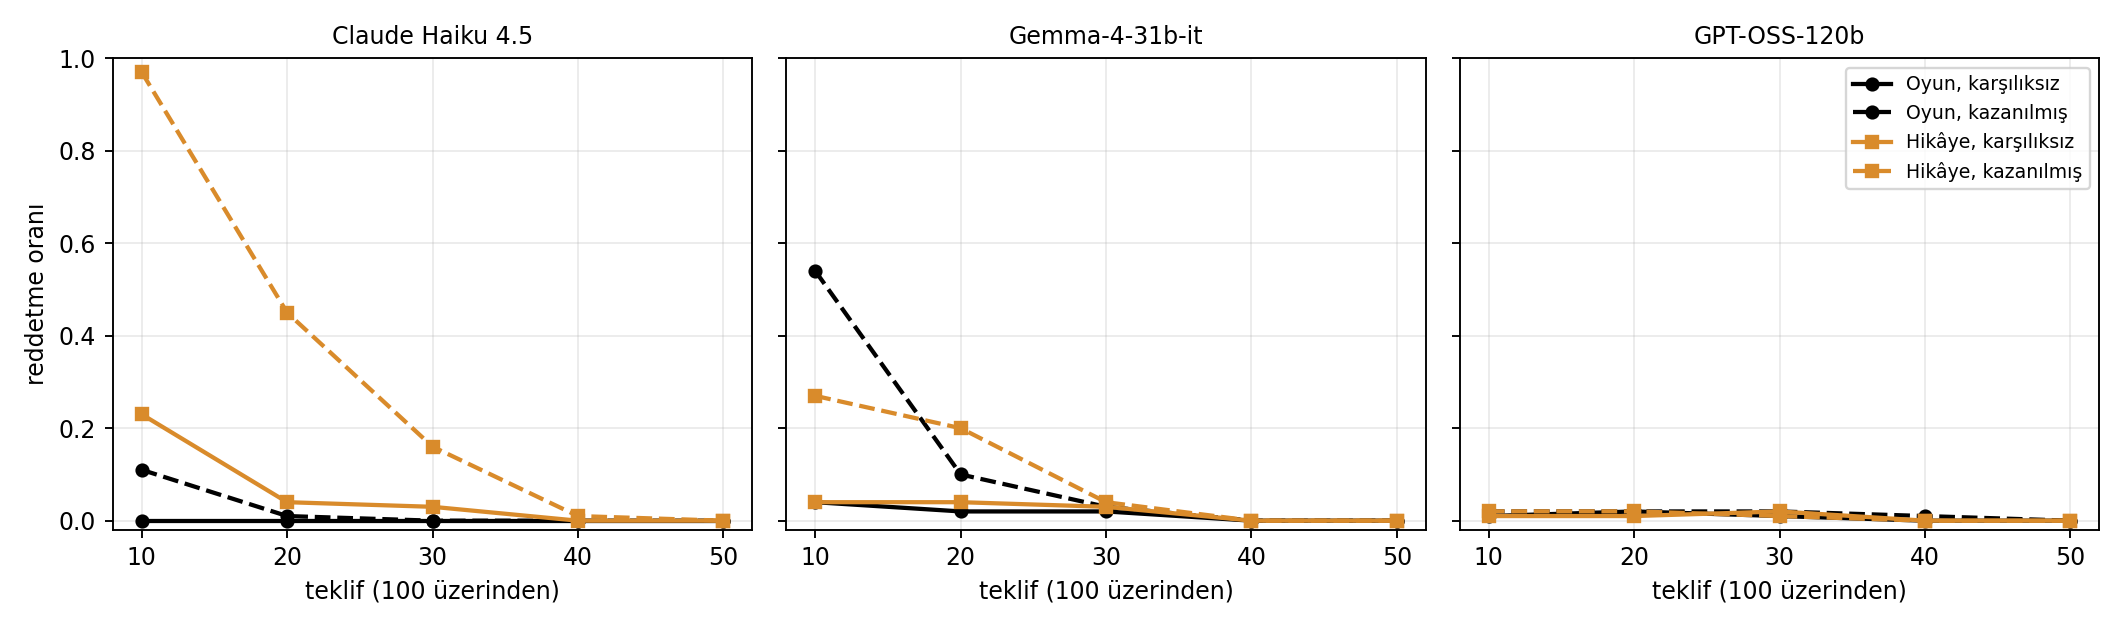
\includegraphics[width=0.98\linewidth]{figs/fig14_entitlement.png}
\caption{Kazanılmış hak testi: teklif düzeyine göre reddetme oranı (kollar havuzlanmış). Kesikli çizgiler havuzun ortak emekle kazanıldığı koşullardır. Haiku ve Gemma'da tek cümlelik emek bilgisi düşük tekliflerde reddetmeyi keskin biçimde artırırken GPT-OSS değişmemektedir.}
\label{fig:entitlement}
\end{figure}

\textbf{Ön kayıtlı hipotez desteklenmiştir.} Havuzun ortak emekle kazanıldığını belirtmek, düşük tekliflerde reddetme oranını oyun çerçevesinde \%1,5'ten \%13,3'e ($+0{,}118$; 73 profil kabulden redde geçmiş, 2 profil ters yönde; $p_{\text{Bonf}} < 10^{-18}$), hikâye çerçevesinde \%6,2'den \%32,3'e ($+0{,}261$; 158'e karşı 2; $p_{\text{Bonf}} < 10^{-43}$) yükseltmiştir. Emek etkisi teklif büyüklüğüyle monoton olarak azalmakta ve \%40--50 tekliflerde kaybolmaktadır; yani modeller herhangi bir bölüşümü değil, emek katkısıyla orantısız bölüşümü reddetmektedir (Şekil~\ref{fig:entitlement}).

Etki modele güçlü biçimde bağlıdır. Haiku, kazanılmış havuzda \%10'luk teklifi hikâye çerçevesinde \%97 oranında reddetmektedir; aynı teklifi standart paradigmada hiç reddetmemiştir. Gemma'da emek bilgisi orijinal oyun metni içinde bile \%10'luk teklifte reddetmeyi \%4'ten \%54'e çıkarmaktadır; bu, Henrich'in WEIRD aralığının (\%40--60) içindedir. GPT-OSS ise dört hücrenin tamamında yaklaşık \%2'de kalmaktadır. Manipülasyon kontrolü, GPT-OSS'un emek bilgisini fark ettiğini göstermektedir: hikâye çerçevesinde kazanılmış koşuldaki gerekçelerin \%48,6'sı emeğe atıf yaparken karşılıksız koşulda bu oran \%0,2'dir. Oyun çerçevesinde bu fark 0,17'dir ve ön kayıtlı 0,20 eşiğinin hemen altındadır. Yani GPT-OSS'un duyarsızlığı bilginin gözden kaçmasından değil, karar kuralının emeğe yanıt vermemesinden kaynaklanmaktadır.

İkincil analizler iki ek örüntü göstermektedir. (i) Çerçeve ile kaynak etkileşmektedir: emek etkisi hikâye çerçevesinde oyun çerçevesine göre daha büyüktür (etkileşim $+0{,}143$). (ii) Karşılıksız havuzda çerçevenin kendisi yalnızca Haiku'da etkilidir (\%0 $\to$ \%13,5; Gemma ve GPT-OSS'ta anlamsız). Bu, gizlenmiş oyun testindeki cüzdan sonucuyla birlikte, gizlemenin tek başına değil, gizlenmiş sahnenin bir ortak etkinlik (``birlikte bulduğumuz meyveler'') ima etmesi ölçüsünde etkili olduğunu düşündürmektedir.

Bu örüntü insan deneylerindeki kazanılmış hak etkileriyle yönsel olarak uyumludur. İnsan katılımcılarda bölüşülecek kaynağın bir çabayla kazanılmış olması, bölüşüm davranışını belirgin biçimde değiştirir: öncelik hakkını bir sınavla kazanan teklif ediciler daha az teklif eder \citep{hoffman1994}; parayı emekle kazanan diktatörler neredeyse hiç pay vermez \citep{cherry2002}; parayı alıcı kazanmışsa diktatörler yarıdan fazlasını bırakabilir \citep{oxoby2008}. Mevcut çalışmada emeği paylaşan yanıtlayıcının orantısız bölüşümü reddetmesi aynı mülkiyet hakkı mantığının yanıtlayıcı tarafındaki karşılığıdır. Ancak bu karşılaştırma yönseldir; insan verisiyle aynı tasarımda nicel bir kalibrasyon yapılmamıştır.


Sayıların etkisinin sınandığı testte (Bölüm~\ref{sec:numbers}) kazanılmış hak etkisi, önceden kayıtlı bir plasebo koşuluyla da karşılaştırılmıştır. Plasebo cümlesi aynı emek dilini kullanmakta, ancak o emeğin havuzla ilgisi olmadığını açıkça belirtmektedir (``that practice task was unpaid and had nothing to do with this money''). Haiku ve Gemma'da emekle kazanılmış havuz plasebodan belirgin biçimde daha fazla reddetme üretmiştir ($+0{,}175$; McNemar $p < 10^{-100}$); dolayısıyla etki yalnızca ``work'' veya ``half'' sözcüklerine verilen bir tepki değildir. Ancak plasebo da karşılıksız havuza göre reddetmeyi bir miktar artırmıştır ($+0{,}081$); önceden yazılan ölçüt ($< 0{,}05$) bu nedenle karşılanmamıştır. Gerekçeler, havuzla ilgisiz ortak bir emeğin de bir karşılıklılık beklentisi yarattığını göstermektedir (``we did equal work yesterday'').




\bibliographystyle{plainnat}
\bibliography{references}

\end{document}
